%-------------------------------------------
% Packages Used
%-------------------------------------------
\documentclass[12pt, a4paper]{article}

% === Basic Document and Encoding ===
\usepackage[T1]{fontenc}        % Font encoding
\usepackage{geometry}           % Page size and margins
\usepackage{setspace}           % Line spacing
\usepackage{lipsum}             % Dummy text

% === Math and Symbols ===
\usepackage{amsmath}            % Math environments
\usepackage{amsfonts}           % Math fonts
\usepackage{mathrsfs}           % Script fonts
\usepackage{eqnarray}           % Eqnarray environment

% === Tables and Tabulars ===
\usepackage{booktabs}           % Professional tables
\usepackage{threeparttable}     % Table footnotes
\usepackage{longtable}          % Long tables
\usepackage{multirow}           % Multirow cells
\usepackage{diagbox}            % Diagonal boxes in tables
\usepackage{tabularray}         % Tabularray tables
\usepackage[table]{xcolor}      % Table cell coloring

% === Figures and Graphics ===
\usepackage{graphicx}           % Images
\usepackage{float}              % Customizing float positions
\usepackage{subcaption}         % Subfigures
\usepackage{caption}            % Caption customization
\usepackage{afterpage}          % Place floats after page break
\usepackage{adjustbox}          % Adjustable boxes for tables and figures

% === Algorithms and Code ===
\usepackage{algorithm}          % Algorithm floats
\usepackage{algorithmicx}       % Algorithmicx package
\usepackage{algpseudocode}      % Pseudocode
\usepackage{listings}           % Code listings

% === Document Structure and Sections ===
\usepackage{titlesec}           % Section formatting
\usepackage[title]{appendix}    % Appendix environment
\usepackage{authblk}            % Author affiliations
\usepackage{chngcntr}           % Change counters

% === Text Formatting and Lists ===
\usepackage{enumitem}           % Custom lists
\usepackage[]{ragged2e}         % Ragged right text
\usepackage{comment}            % Large comment blocks

% === Landscape and Page Layout ===
\usepackage{lscape}             % Landscape tables
\usepackage{pdflscape}          % Landscape pages

% === Bibliography and Citations ===
\usepackage[backend=biber, citestyle=apa, bibstyle=apa, maxbibnames=20, date=year, urldate=year, alldates=year]{biblatex} % Bibliography management
\usepackage{csquotes}           % Context-sensitive quotation

% === Hyperlinks and Colors ===
\usepackage[colorlinks=true, allcolors=blue]{hyperref} % Hyperlinks

% === Miscellaneous ===
\usepackage{orcidlink}          % ORCID iDs
\usepackage{lineno}             % Line numbers
% \usepackage[none]{hyphenat}     % Disable hyphenation
\usepackage{csvsimple}          % Import CSV to LaTeX

%-------------------------------------------
% Document Preamble
%-------------------------------------------

% === Bibliography Reference ===
\addbibresource{refs.bib} % Reference .bib file
%\bibliographystyle{apa}

% === Page Layout and Spacing ===
\geometry{a4paper,
        top=1in,
        bottom=1in,
        left=1in,
        right=1in,
        marginparwidth=0.5in
        }

\onehalfspacing % 1.5 line spacing
\setlength{\parskip}{0.5\baselineskip} % Vertical space between paragraphs
\setlength{\parindent}{1.5em} % Paragraph indentation

% === Section Formatting ===
\titleformat{\section} % Redefine section numbering format
{\normalfont\Large\bfseries}{\thesection.}{1em}{}

% === Line Numbering ===
% \renewcommand\linenumberfont{\normalfont\scriptsize\sffamily\color{blue}}
% \linenumbers % Enable line numbering
% \rightlinenumbers % Right-align; comment this line for left alignment.

% === Custom Commands and Environments ===
% Define a new command for the fourth-level title.
\newcommand{\subsubsubsection}[1]{%
  \vspace{\baselineskip} % Add some space
  \noindent\textbf{#1\\}\quad % Adjust formatting as needed
}

% Change the position of the table caption above the table
\captionsetup[table]{position=top} % caption position for tables

% Make Table and Figure labels bold and change separator from colon to period
\captionsetup{labelfont=bf, labelsep=period} % Make all caption labels (Table X, Figure X) bold and use period separator

% Define the unnumbered list
\makeatletter
\newenvironment{unlist}{%
  \begin{list}{}{
    \setlength{\labelwidth}{0pt}%
    \setlength{\labelsep}{0pt}%
    \setlength{\leftmargin}{2em}%
    \setlength{\itemindent}{-2em}%
    \setlength{\topsep}{\medskipamount}%
    \setlength{\itemsep}{3pt}%
  }%
}{%
  \end{list}%
}
\makeatother


% === Miscellaneous Settings ===
% Suppress the warning about \@parboxrestore
%\pdfsuppresswarningpagegroup=1

% Suppress the warning about overfull boxes
\sloppy

%-------------------------------------------
% Title and Abstract
%-------------------------------------------
\title{\textbf{Are Older Adults in China Living Longer Happy Years? A Cohort-Based Multistate Analysis, 2002–2018}}
\author[]{Yunxiang Wan} %\orcidlink{0009-0003-7482-7991}

%\affil[1]{\small{Max Planck Institute for Demographic Research, Rostock, Germany, 18057}}
%\affil[2]{\small{French Institute for Demographic Studies, Paris, France, 93300}}
%\affil[3]{\small{Max Planck Institute for Demographic Research, Rostock, Germany, 18057}}
%\affil[*]{Corresponding author: \href{mailto:wan@demogr.mpg.de}{wan@demogr.mpg.de}}
\date{}

\begin{document}
\newpage

% === Title ===
\maketitle

\begin{center}
  {EDSD mentors: Marília Nepomuceno, Marwân-al-Qays Bousmah}
\end{center}
\vspace{1em}

% === Abstract ===
\begin{abstract}
  \noindent\textbf{Objective:} As China’s population ages and life expectancy rises, a critical question remains: are these added years also happy years? This study assesses cohort trends in happy life expectancy (HapLE) and quantifies how socioeconomic disparities in these trends have evolved.

  \noindent\textbf{Methods:} Using data from the Chinese Longitudinal Healthy Longevity Survey (CLHLS, 2002–2018), we applied multistate life tables to estimate partial-cohort HapLE (PC-HapLE) across four age ranges. We compared earlier cohorts with later cohorts born 10 years apart, stratifying analyses by gender, education, and urban-rural residence.

  \noindent\textbf{Results:} Later-born cohorts experienced a significant increase in both the number and proportion of happy years, driven by a "compression of unhappiness." However, these gains were unequally distributed. Gains in PC-HapLE were substantial and significant for urban older adults across all age ranges, whereas those for rural residents were modest and often statistically insignificant. This pattern of widening inequality was mirrored by education and gender, with literate individuals and women showing greater improvements.

  \noindent\textbf{Conclusion:} Although later cohorts of Chinese older adults are living longer happy years, this aggregate improvement conceals a widening "happiness gap." The benefits of socioeconomic development have disproportionately accrued to urban, educated, and female populations. Policies must shift from merely extending lifespan to promoting equitable aging by actively addressing these growing disparities.
  \vspace{1em}

  \noindent\textbf{Keywords}: Happy life expectancy, Cohort analysis, Population aging, Socioeconomic disparities, China
\end{abstract}


%-------------------------------------------
% Highlights
%-------------------------------------------
% \newpage
% \section*{Highlights}
% \begin{itemize}
%     \item Problem and solution
%     \item Method
%     \item Result 1 / Recommendations / Policy Implications
%     \item Result 2 / Recommendations / Policy Implications
%     \item Result 3 / Recommendations / Policy Implications / Conclusion
% \end{itemize}

%-------------------------------------------
% Introduction
%-------------------------------------------
\newpage
\section{Introduction}
Over the past few decades, China has undergone a rapid process of population aging. In 2023, the number of individuals aged 65 and older reached 210 million, accounting for more than 15.3\% of the total population, a proportion that has doubled in just over two decades \autocite{nationalbureauofstatisticsofchina.2023.china}. Projections estimate this figure will climb to 390 million by 2050, comprising nearly 30\% of the nation's population \autocite{unitednations.2024.world}.  This demographic shift has been accompanied by increases in life expectancy (LE). In 2023, LE at birth in China stood at 78.0 years, up from just 43.8 years in 1950. Over the same period, LE at age 65 nearly doubled, rising from 9.1 years in 1950 to 17.5 years in 2023 \autocite{unitednations.2024.world}. However, these gains in longevity raise a critical question: are these added years of life also high-quality years? Answering this is crucial for shaping effective aging policies that move beyond merely extending longevity to enhancing the quality of those added years.

To assess the quality of added life-years, scholars have developed summary measures that integrate quantity and quality of life. The most established of these, healthy life expectancy (HLE), decomposes total LE into years lived in good and poor health \autocite{sanders.1964.measuring}. This measure has been instrumental in the long-standing debate on whether populations are experiencing a "compression of morbidity", where longer lives are accompanied by a shorter period of ill-health before death \autocite{fries.1980.aging}—or an "expansion of morbidity," where the extra years are spent in poorer health\autocite{gruenberg.1977.failures}. However, while health is a fundamental component of life quality, it does not encompass the full spectrum of it \autocite{yang.2008.long}. Recognizing this, the World Health Organization defines quality of life as a broad concept encompassing not only physical health but also psychological states and social relationships \autocite{thewhoqolgroup.1998.development}. Happiness is a cognitive, global judgment of the quality of life, which is defined as the extent to which an individual positively evaluates their overall life as a whole \autocite{veenhoven.1996.study}. As an analogy and complement to HLE, happy life expectancy (HapLE) has emerged as a summary measures that integrates longevity with happiness, which reflects not only how long people live but also how long they live in a happy state. By examining HapLE, we can move beyond the narrow focus on disease and disability to assess whether societies are fostering environments where older adults not only survive but also thrive \autocite{yang.2008.long}.

The development of HapLE raises a critical question: as people living longer, are they universally succeeding in converting longer lives into happier ones? Global research on HapLE trends reveals a complex picture. Early research from the United States painted an optimistic narrative of progress, finding that between 1970 and 2000, Americans were living both more years and a larger proportion of their lives happily \autocite{yang.2008.long,yang.2010.increment}. This "compression of unhappiness" was also documented in the Netherlands \autocite{perenboom.2004.trends}. However, this narrative of progress has been challenged. Research in West Germany revealed a paradox: while absolute happy years increased, the proportion of life spent satisfied actually declined due to a deterioration in end-of-life well-being \autocite{nemitz.2022.increasing}. Moreover, HapLE trends in post-communist nations like Russia have been highly volatile, fluctuating with socioeconomic turmoil \autocite{minagawa.2022.trends}. These diverging international findings underscore that HapLE trends are not monolithic but are deeply embedded in national contexts.

The case of China provides a compelling landscape for understanding HapLE dynamics. The country's path has been marked by the "Easterlin paradox"—the observation that massive economic growth may not lead to a corresponding rise in life satisfaction \autocite{easterlin.1974.does}. This phenomenon was prominent in China from the 1990s to the early 2000s, often attributed to the social disruptions of market reforms\autocite{easterlin.2012.chinas,graham.2017.happiness,knight.2011.does}. More recent evidence, however, suggests a reversal of this trend since the early 2000s, with happiness levels rising in tandem with the maturation of China’s social security systems \autocite{cai.2023.does,wang.2023.hierarchical}. Mirroring this positive aggregate trend, the study on HapLE trends in China, a period-based analysis by Duan and Chen \autocite{duan.2020.happy}, documented an overall "compression of unhappiness." However, this narrative of aggregate improvement may conceal possible inequalities in these dynamics. Socioeconomic status acts as a fundamental cause of life chances, shaping access to the resources required for a happy and healthy life \autocite{link.1995.social}. In China, the most prominent fault line is the institutionalized urban-rural divide, which creates significant gaps in income, healthcare, and educational opportunities \autocite{guo.2024.regional,liu.2019.are}. Alongside this, education serves as another key stratifying mechanism, equipping individuals with the knowledge and capital to better manage their lives in a complex society \autocite{cheng.2021.sociodemographic}. A recent analysis of HapLE in China confirmed that disparities exist, with urban and more educated older adults living significantly longer happy lives \autocite{wan.2024.socioeconomic}.

Two important gaps can be identified from the existing literature. First, the reliance on period-based analyses provides an incomplete examination. Period estimates, which aggregate data across cohorts at a single point in time, are useful for monitoring population-level shifts but do not fully capture the lived experiences of actual generations \autocite{payne.2022.expansion}. A cohort perspective is essential to examine whether later-born Chinese are living longer happy lives than their predecessors. Second, while research has established the existence of significant socioeconomic disparities in HapLE at a single period of time \autocite{wan.2024.socioeconomic}, these static analyses leave a crucial question unanswered: have these "happiness gaps" narrowed or widened across cohorts? A dynamic analysis, which examines trends in inequality, is required to assess whether the benefits of China's development have been distributed equitably or have disproportionately favored those with more resources \autocite{liu.2019.are}.

To address these limitations, this study poses two research questions. First, from a cohort perspective, are later-born older Chinese adults living more happy years than their predecessors? Second, how have socioeconomic disparities in HapLE—specifically by education, urban-rural residence, and gender—evolved across these successive birth cohorts? In other words, have these "happiness gaps" widened or narrowed over time? To answer these questions, we employ a cohort-based multistate life table approach using nationally representative data from the Chinese Longitudinal Healthy Longevity Survey (CLHLS) from 2002 to 2018. By investigating both the overall cohort trend and its inequalities, this study aims to provide a more comprehensive understanding of population life quality in aging China.

%-------------------------------------------
% Method
%-------------------------------------------

% === Data ===
\section{Method}
\subsection{Data}
This study used data from CLHLS, a longitudinal study of older adults in China \autocite{centerforhealthyaginganddevelopmentstudies.2020.chinese}. The CLHLS covers 23 of China’s 31 provinces, municipalities, and autonomous regions, accounting for approximately 85\% of the nation's total population, making it a robust data source for examining trends in aging \autocite{gu.2008.general,zeng.2008.introduction}. The survey was initiated in 1998 and has since conducted eight waves of follow-up, spanning two decades. While the initial waves targeted individuals aged 80 and above, the survey expanded its scope from 2002 onwards to include those aged 65 and older. Our analysis drew upon two distinct observation periods to construct and compare successive birth cohorts. The earlier cohort sample (N = 7,275) was derived from individuals who participated in the 2002 baseline wave and had at least one follow-up observation in either the 2005 or 2008 waves, including those confirmed to have died during this period. Similarly, the later cohort sample (N = 4,759) comprised participants from the 2011/2012 baseline wave (hereafter, the 2012 wave) who had at least one follow-up observation in the 2014 or 2017/2018 waves (hereafter, the 2018 wave), or were confirmed deceased.

% === Measures ===
\subsection{Measures}
This study used HapLE as the outcome to examine cohort trends in longevity and happiness among older adults in China. By decomposing LE into the number of years lived in happy and unhappy states, both HapLE and unhappy life expectancy (UHapLE) can be derived. HapLE and UHapLE can be viewed from an absolute perspective, referring to the number of years an individual is expected to live in a happy state, or from a relative perspective, as the proportion of HapLE in LE (HapLE\%) and UHapLE in LE (UHapLE\%), respectively.

Happiness was assessed using a single-item measure of life satisfaction in CLHLS. The terms subjective well-being, life satisfaction, and happiness are often considered interchangeable in relevant literature \autocite{easterlin.2021.growth,yang.2008.long}. This measurement approach has been widely applied in large-scale surveys due to its simplicity and effectiveness and has demonstrated high reliability and validity in assessing individual well-being \autocite{baur.1983.stability,lucas.2018.shortterm}. Specifically, CLHLS evaluated respondents' life satisfaction through the question: "How do you feel about your life at present?" Responses were rated on a five-point scale. In line with previous research \autocite{duan.2020.happy,wan.2024.socioeconomic}, we dichotomized the variable for analytical purposes: respondents answering "very good" or "good" were classified as "happy," while those answering "so so", "bad" or "very bad" were categorized as "unhappy." Mortality information in CLHLS was primarily obtained from official death certificates. In their absence, data were collected from local residential committees or reports from close relatives. When a respondent's death was confirmed in a specific survey wave, their survival status in that wave was recorded as "dead."

This study included five covariates: age, sex, birth cohort, urban-rural residence, and education level. Education level is a well-established indicator of socioeconomic status and serves as a key predictor of an individual's social and economic conditions \autocite{kwok.2001.use}. Urban-rural residence is closely linked to inequalities in healthcare access, income levels, economic growth, and infrastructure development in Chinese society, which have been extensively studied \autocite{liu.2019.are}. In this study, education attainment and urban-rural residence were further used in subgroup analyses. Age was treated as a continuous variable, and sex was categorized as men or women. Birth cohort was operationalized as a comparative variable distinguishing between an "earlier cohort" and a "later cohort" within each age range. A detailed description of the cohort design is provided in the Analyses section (Table 1). Urban-rural residence was measured at baseline using the survey question: "Where do you currently live?" Response options included "city," "town," and "rural area." In this analysis, the "city" and "town" categories were combined into "urban." Educational level was coded based on respondents' years of schooling at baseline, derived from the survey question: "How many years of formal education have you completed in total?" Respondents with zero years of schooling were classified as "illiterate," while those with more than zero years were categorized as "literate."

% === Analyses ===
\subsection{Analyses}
This study used a method for estimating state-specific partial-cohort life expectancy (PC-LE), which calculates total LE within a specified age range for a given cohort, as well as the expected years lived in a specific state (e.g., happy). This method had been used to examine trends in healthy life expectancy (HLE), disability-free life expectancy (DFLE), and morbidity-free life expectancy (MFLE) across successive birth cohorts \autocite{liu.2019.are,payne.2022.expansion,payne.2019.expansion,shen.2023.disability}. Compared to estimates of full-cohort life expectancy, PC-LE estimates do not require data from fully extinct cohorts, making them more practical for contemporary demographic analyses. Furthermore, using cohort-based estimates helps mitigate biases arising from structural changes across generations, thereby providing clearer comparisons between different population groups \autocite{payne.2022.expansion}.

% === Table 1 ===
\begin{table}[htbp]
  \centering
  \caption{Information on age-group, period, and birth cohort comparisons}
  \begin{tabular}{cccc}
    \toprule
    \multirow{3}{*}{\text{Age Range}} &  & \multicolumn{2}{c}{\text{Period}}                     \\
    \cmidrule(lr){3-4}
                                      &  & \text{2002--2008}                 & \text{2012--2018} \\
                                      &  & Earlier cohort                    & Later cohort      \\
    \midrule
    68--73                            &  & 1932--1937                        & 1942--1947        \\
    74--79                            &  & 1926--1931                        & 1936--1941        \\
    80--85                            &  & 1920--1925                        & 1930--1935        \\
    86--91                            &  & 1914--1919                        & 1924--1929        \\
    \bottomrule
  \end{tabular}
\end{table}

Table 1 presents information on the eight period–cohort groupings analyzed in this study. Our primary focus is to compare PC-LE and partial-cohort happy life expectancy (PC-HapLE) within four independent 6-year age ranges (68-73, 74-79, 80-85, and 86-91) \footnote{Two higher age ranges (92–97 and 98–103) were also analyzed but excluded from the final models. This decision was due to insufficient statistical power, stemming from small sample sizes and a low number of observed transitions between happiness states, which resulted in unreliable model estimates and non-significant overall model fit.} across two successive birth cohorts born 10 years apart (referred to as "earlier" and "later" cohorts). Figure 1 provides a Lexis diagram to illustrate this structure for the 68–73 age range. For each comparison, our models use all observed data for members of a given birth cohort during its corresponding observation period. For example, to compare happiness in the 68-73 age range, we analyze the cohort born 1932–1937 (observed in 2002–2008) and the cohort born 1942–1947 (observed in 2012–2018). To enhance interpretability and account for potential age composition variations within these 6-year birth cohorts, we predict transition probabilities and estimate PC-LE and PC-HapLE for the central age-trajectory in each range. As illustrated by the diagonal dashed line in Figure 1, this means that for the 68–73 age range comparison, expectancies are estimated for each cohort over the 6-year span starting at exact age 68 and ending at exact age 74.

% === Figuere 1 ===
\begin{figure}[htbp]
  \centering
  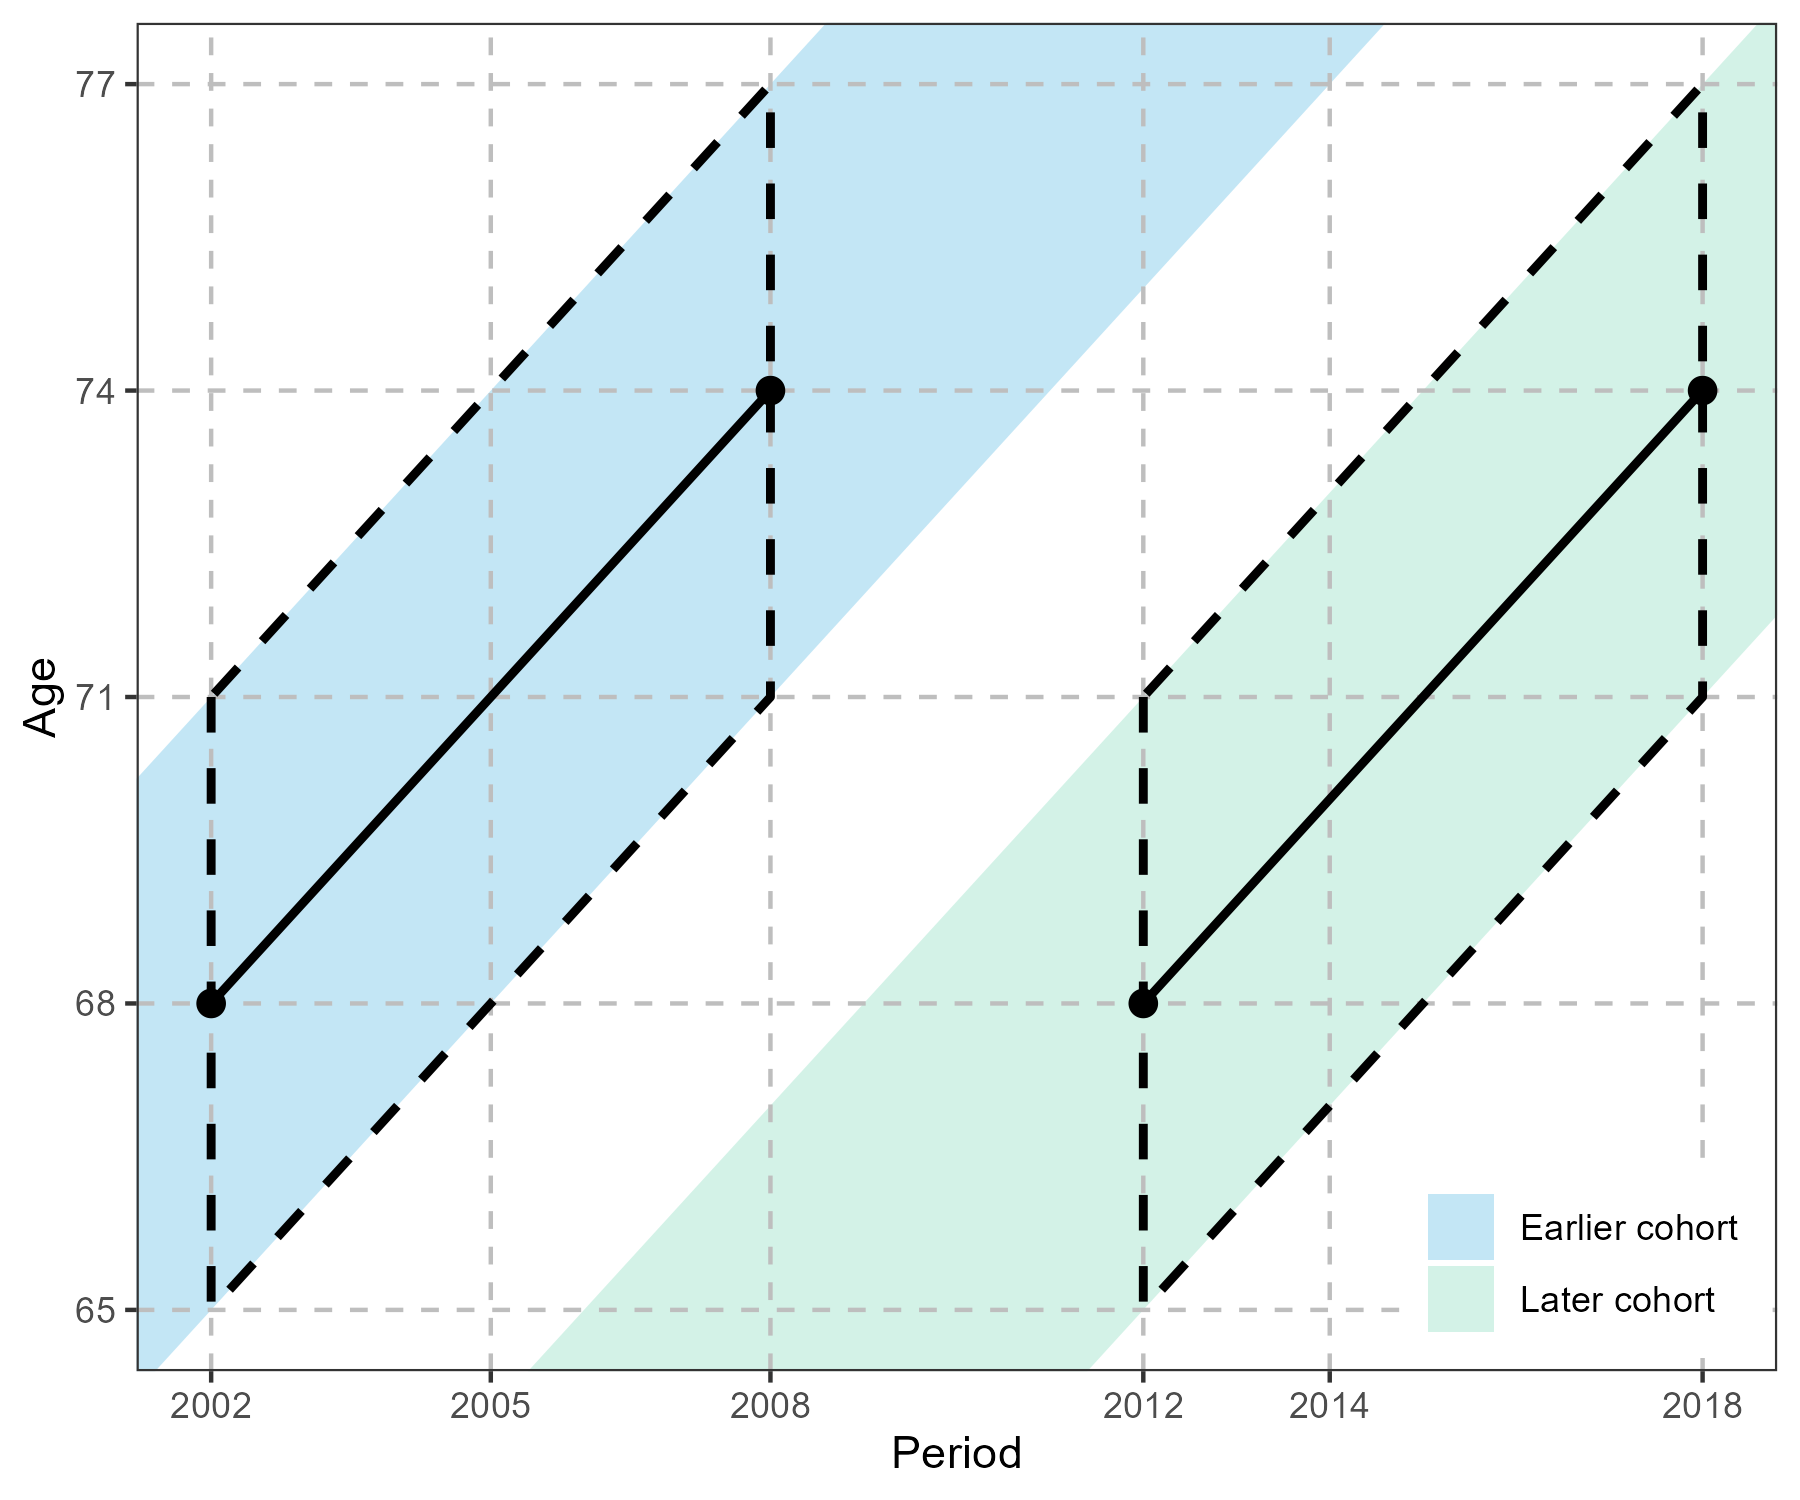
\includegraphics[width=0.8\textwidth]{fig_tabs_b300/2_1_Lexis_Diagram.png}
  \caption{Lexis diagram used for cohort comparisons in the 68-73 age range}
  \label{fig:Lexis_Diagram}
\end{figure}

This study applied the MSLT method to estimate PC-LE and PC-HapLE. As shown in Figure 2, three discrete states were defined: happy, unhappy, and dead. Four potential transitions were considered: happy to unhappy, unhappy to happy, happy to dead, and unhappy to dead. The estimation of MSLT functions was performed using a modified version of the Stochastic Population Analysis for Complex Events (SPACE) program \autocite{cai.2010.estimation} in SAS 9.4 \autocite{sasinstituteinc..2016.sas}. Subsequent data processing and all visualizations were conducted in R \autocite{rcoreteam.2023.language}.

The SPACE computation process consisted of three sequential steps. First, data preprocessing was conducted to accommodate the varying intervals between CLHLS survey waves. SPACE converted CLHLS data into person-years format and imputed annual state values, filling missing years with pseudo-data to represent consecutive years of observation. Second, annual transition probabilities were estimated for each age range using multinomial logistic regression. The base model incorporated age, age-squared, sex, cohort, and interactions between age, sex, and birth cohorts. Two additional models were fitted to examine subgroup differences: one incorporating education level and another including urban-rural residence, along with their respective interaction terms with age, sex, and cohort. Third, microsimulation was employed to compute PC-LE and PC-HapLE based on the estimated transition probability matrices. A synthetic cohort of 100,000 individuals was created, with each person assigned an initial happiness state according to the weighted distribution observed at the starting age of each age range. Annual transitions were simulated by comparing random uniform numbers against age-specific transition probabilities until individuals reached the upper bound of their respective age range. PC-LE was calculated as the mean survival years within the age range, while PC-HapLE represented the mean years spent in the happy state. Confidence intervals were derived through bootstrap resampling with 300 iterations to capture uncertainty in both parameter estimation and microsimulation processes.

% === Figure 2 ===
\begin{figure}[htbp]
  \centering
  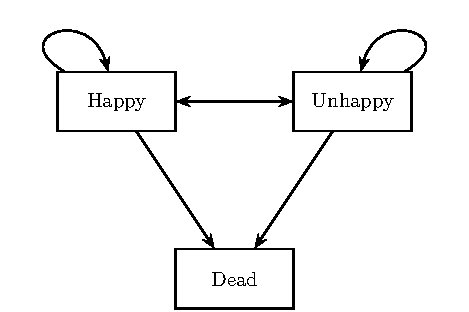
\includegraphics[width=0.8\textwidth]{fig_tabs_b300/latex_output/State_space.pdf}
  \caption{State space in the multi-state model}
  \label{fig:State_space}
\end{figure}

Inverse probability weighting (IPW) was applied to adjust for potential biases arising from differential loss to follow-up. This method assigned higher weights to individuals who completed follow-up, where weights were inversely proportional to the probability of completing follow-up. The probability models included all sociodemographic and a disability variable measured by Activities of Daily Living (ADL) \autocite{payne.2022.expansion,liu.2019.are,shen.2023.disability}. IPW weights were estimated separately for each period and birth cohort, and the final analytical weight was derived by multiplying the IPW weight by the combined respondent weight from CLHLS \autocite{dugoff.2014.generalizing,liu.2019.are}.

To test the robustness of our findings to the dichotomization of the happiness variable, we conducted a sensitivity analysis. In this analysis, we re-specified the outcome variable using a three-category measure based on the original five-point scale: "happy" (comprising "very good" and "good" responses), "neutral" (comprising "so so" responses), and "unhappy" (comprising "bad" and "very bad" responses). This resulted in a four-state model that included transitions among happy, neutral, unhappy, and dead states\footnote{We present this as a sensitivity analysis rather than our primary model for two main reasons. First, the "unhappy" state in the four-state model has a small sample size (as shown in Table S1), which could affect the statistical power and stability of the transition probability estimates. Second, the main three-state model ensures consistency with prior literature, facilitating direct comparisons.}, as shown in the Appendix Figure S1. Consequently, in addition to PC-HapLE and PC-UnHapLE, this model allowed us to estimate partial-cohort neutral life expectancy (PC-NLE), defined as the expected number of years lived in a "neutral" state within each age range. The models were re-estimated using this expanded state space, following the same analytical procedures described above.

%-------------------------------------------
% Results
%-------------------------------------------
\section{Results}
The Appendix Table S1 presents the baseline characteristics of each birth cohort within the four age ranges examined in this study. Gender distribution remained relatively stable across cohorts, with men comprising approximately 50\%-56\% of each cohort. There was a clear trend of increasing educational attainment across most age ranges, with the proportion of literate individuals rising notably in younger age ranges but showing mixed patterns in older ranges. Urban-rural residence distribution varied across cohorts without consistent patterns. Baseline happiness levels showed mixed patterns across age ranges, with modest changes ranging from slight decreases to small increases across cohorts.

% === 3.1 ===
\subsection{Overall Cohort Differences in PC-LE and PC-HapLE}

Figure 3 and the Appendix Table S2 present estimated partial-cohort life expectancy (PC-LE), partial-cohort happy life expectancy (PC-HapLE), and partial-cohort unhappy life expectancy (PC-UnHapLE) across birth cohorts for four age ranges (68–73, 74–79, 80–85, and 86–91). Overall, later-born cohorts of Chinese older adults experienced significant increases in both the absolute number and relative proportion of happy years, accompanied by a compression of unhappy years.

Across all age ranges examined, PC-HapLE increased substantially between earlier and later cohorts, with gains ranging from 0.39 to 0.60 years. The most pronounced improvements occurred in the youngest age range (68–73), while significant increases were also observed in all older age ranges. These gains in happy years were accompanied by corresponding significant reductions in PC-UnHapLE across all age ranges, with the largest decreases observed in the youngest age range. The relative improvements were equally striking, with HapLE\% rising substantially across cohorts, ranging from 7.0 to 11.5 percentage points, with the greatest increases in the youngest age range. Meanwhile, total PC-LE remained largely stable across cohorts in most age ranges, with only modest and generally non-significant changes observed, except for a small but significant increase of 0.21 years in the oldest age range (86-91).

% === Figure 3 ===
\begin{figure}[!p]
  \centering
  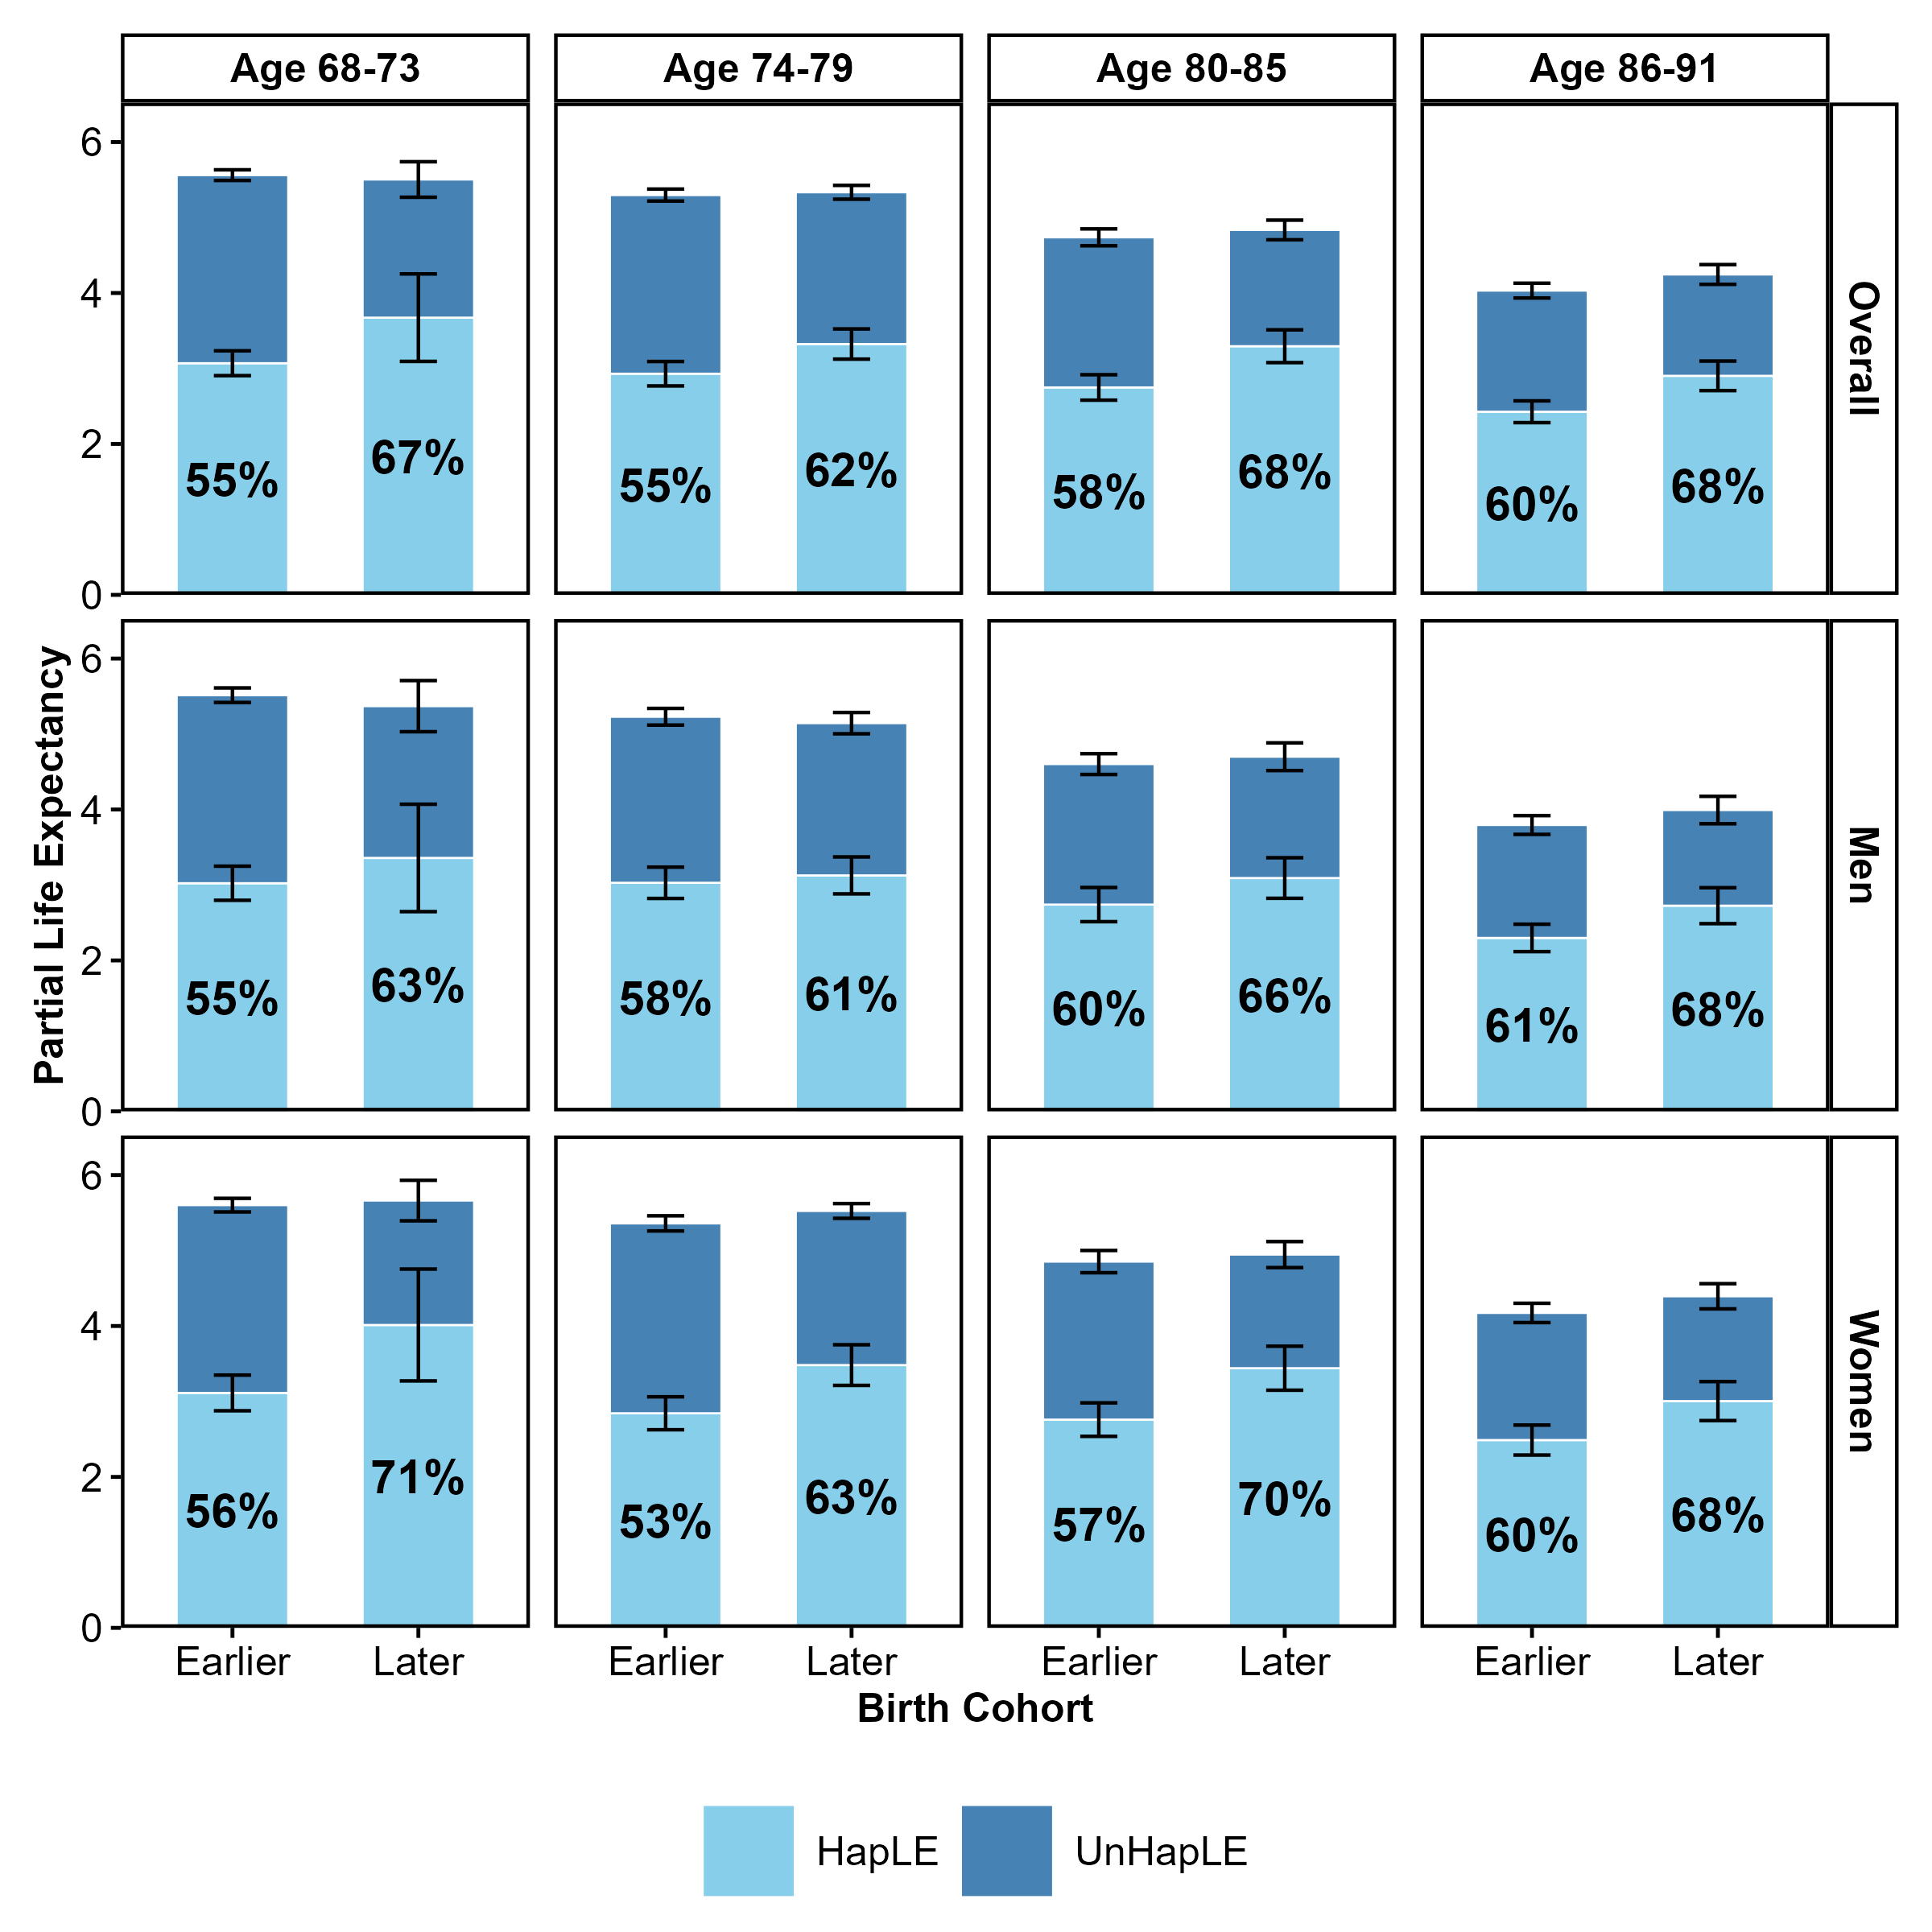
\includegraphics[width=1\textwidth]{fig_tabs_b300/2_2_HapLE_stacked_plots_sex.png}
  \caption{Estimated PC-LE, PC-HapLE and PC-UnHapLE by age range, birth cohorts and sex. \textbf{Notes}: Each bar represents PC-LE for a specific birth cohort, age range, and sex. The bar is divided into PC-HapLE (light shading) and PC-UnHapLE (dark shading). The figure inside each bar indicates HapLE\%. Black vertical lines represent the 95\% CI for the PC-LE and PC-HapLE estimates. Values of estimates can also be found in Appendix Table S2. \textbf{Source}: Author's calculation based on CLHLS, 2002–2018.}
\end{figure}

% === 3.2 ===
\subsection{Cohort Differences in PC-LE and PC-HapLE by Gender}

Figure 3 and Table S2 also show substantial gender disparities in cohort changes of PC-HapLE. Older women experienced consistently larger and more statistically significant improvements in PC-HapLE and HapLE\% compared to men across most age ranges.

Among women, significant increases in PC-HapLE were observed across all four age ranges, ranging from 0.52 to 0.90 years, with the largest improvements in the youngest age range (68–73). These gains were accompanied by corresponding significant reductions in PC-UnHapLE and substantial increases in HapLE\%, with improvements ranging from 8.8 to 15.3 percentage points across age ranges. PC-LE among women remained relatively stable or showed modest increases, with a statistically significant increase observed only in the 74–79 age range. In contrast, men demonstrated more modest and less consistent gains. Statistically significant increases in PC-HapLE among men were observed only in the two oldest age ranges (80–85 and 86–91), with gains of approximately 0.35-0.43 years. For the younger age ranges (68–73 and 74–79), while point estimates suggested modest improvements, the changes did not reach statistical significance due to considerable uncertainty. PC-LE among men also remained largely stable across most age ranges. These contrasting patterns resulted in substantially larger proportional gains in HapLE\% for women compared to men across all age ranges.

% === 3.3 ===
\subsection{Cohort Differences in PC-LE and PC-HapLE by Education}

As detailed in Figure 4 and the Appendix Table S3, there were significant differences in PC-HapLE between literate and illiterate older adults across most age ranges. Literate older adults consistently experienced larger and more statistically significant gains in PC-HapLE and HapLE\% compared to their illiterate counterparts across most age ranges examined.

Among literate older adults, significant increases in PC-HapLE were observed in three age ranges (74-79, 80-85, and 86-91), ranging from 0.47 to 0.72 years, with the largest gains in the 80–85 age range. These improvements were accompanied by corresponding significant reductions in PC-UnHapLE and substantial increases in HapLE\%, most notably a 14.4 percentage point increase in ages 80–85. PC-LE among literate adults remained relatively stable across most age ranges, with only the oldest age range (86–91) showing a significant increase. In contrast, illiterate older adults showed smaller and less consistent improvements. Statistically significant increases in PC-HapLE were observed only in the two oldest age ranges (80–85 and 86–91), with gains of approximately 0.35-0.40 years. For the younger age ranges (68–73 and 74–79), while point estimates suggested modest improvements, the wide confidence intervals indicated considerable uncertainty, and the changes did not reach statistical significance. PC-LE among illiterate adults also remained largely stable across age ranges. These divergent patterns resulted in much larger proportional gains in HapLE\% for literate compared to illiterate older adults across most age ranges.

% === Figure 4 ===
\begin{figure}[!p]
  \centering
  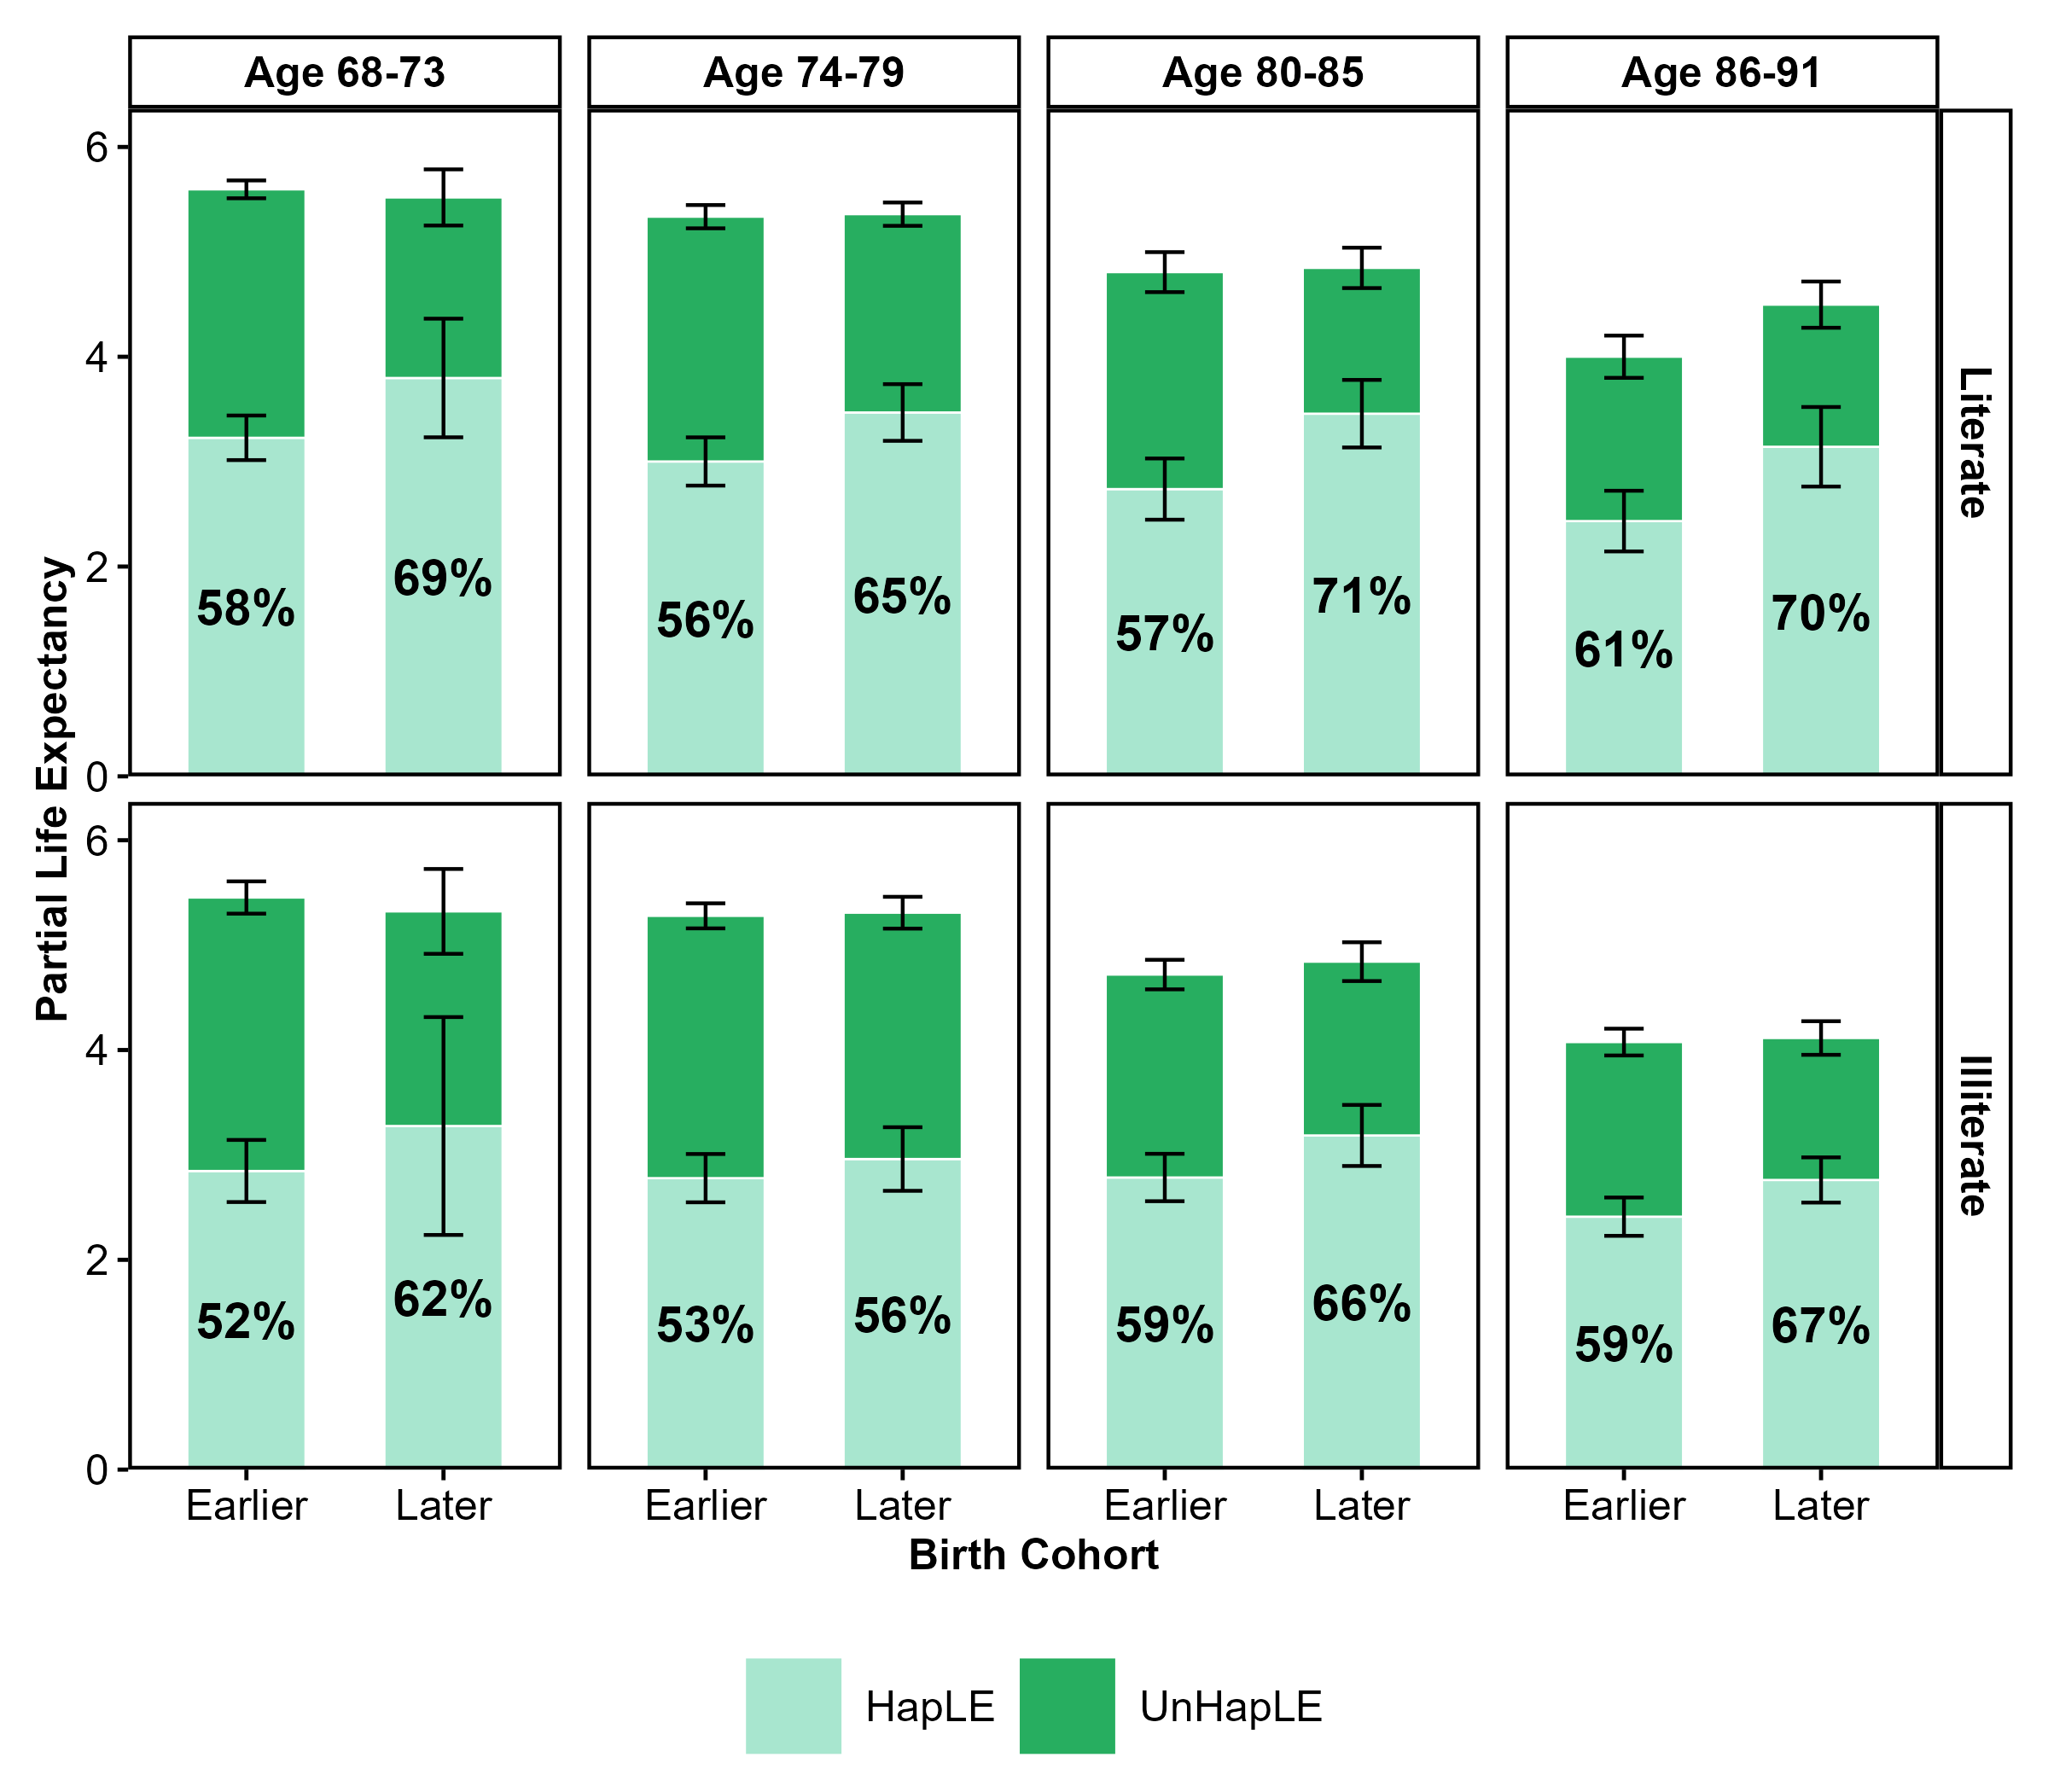
\includegraphics[width=1\textwidth]{fig_tabs_b300/2_3_HapLE_stacked_plots_edu.png}
  \caption{Estimated PC-LE, PC-HapLE and PC-UnHapLE by age range, birth cohorts and education level. \textbf{Notes}: Each bar represents PC-LE for a specific birth cohort, age range, and education level. The bar is divided into PC-HapLE (light shading) and PC-UnHapLE (dark shading). The figure inside each bar indicates HapLE\%. Black vertical lines represent the 95\% CI for the PC-LE and PC-HapLE estimates. Values of estimates can also be found in Appendix Table S3. \textbf{Source}: Author's calculation based on CLHLS, 2002–2018.}
\end{figure}

% === 3.4 ===
\subsection{Cohort Differences in PC-LE and PC-HapLE by Residence}

The most pronounced disparities in cohort trends were observed between urban and rural residents (Figure 5 and the Appendix Table S4). Urban older adults experienced substantial and highly significant improvements in PC-HapLE and HapLE\% across all age ranges, while rural residents showed more modest and inconsistent gains.

Among urban residents, significant increases in PC-HapLE were observed across all four age ranges, ranging from 0.46 to 1.04 years, with the largest gains in the youngest age range (68–73). These improvements were accompanied by corresponding significant reductions in PC-UnHapLE and substantial increases in HapLE\%, most notably a 16.9 percentage point increase in ages 68–73. PC-LE among urban residents remained relatively stable, with modest increases observed in most age ranges, particularly a significant increase in the oldest age range (86–91). In contrast, rural residents showed a markedly different pattern. Statistically significant increases in PC-HapLE were observed only in the two oldest age ranges (80–85 and 86–91), with gains of approximately 0.43-0.45 years. For the younger age ranges (68–73 and 74–79), while point estimates suggested modest improvements, the wide confidence intervals indicated considerable uncertainty, and the changes did not reach statistical significance. PC-LE among rural residents also remained largely stable across most age ranges. These divergent patterns resulted in much larger proportional gains in HapLE\% for urban residents compared to their rural counterparts across all age ranges.

% === 3.5 ===
\subsection{Sensitivity Analysis}

A sensitivity analysis was conducted to test the robustness of our findings to the dichotomization of the happiness variable, using a three-category happiness measure. The detailed estimates, presented in Appendix Tables S5–S7, strongly corroborated our primary conclusions.

First, the analysis re-comfirmed the overall trend of a "compression of unhappiness." Later-born cohorts demonstrated significant increases in PC-HapLE, which the four-state model revealed was driven by both significant reductions in years spent in the 'unhappy' state (PC-UnHapLE) and a concurrent, significant compression of years spent in the 'neutral' state (PC-NLE) (Table S5). Second, the analysis reinforced the finding of a widening "happiness gap" across subgroups. Consistent with our main findings, older women and literate individuals experienced larger and more statistically significant improvements in PC-HapLE and HapLE\% compared to men and their illiterate counterparts (Tables S5 \& S6). This advantage was primarily driven by a significant compression of both their unhappy and neutral years. The pattern of widening inequality was most pronounced between urban and rural residents (Table S7). Urban older adults saw substantial and highly significant increases in PC-HapLE, attributable to reductions in both PC-NLE and PC-UnHapLE. In contrast, gains for their rural counterparts remained modest and were largely statistically non-significant. In sum, these results confirm that our study's core conclusions are robust and not an artifact of the measurement strategy.

% === Figure 5 ===
\begin{figure}[!p]
  \centering
  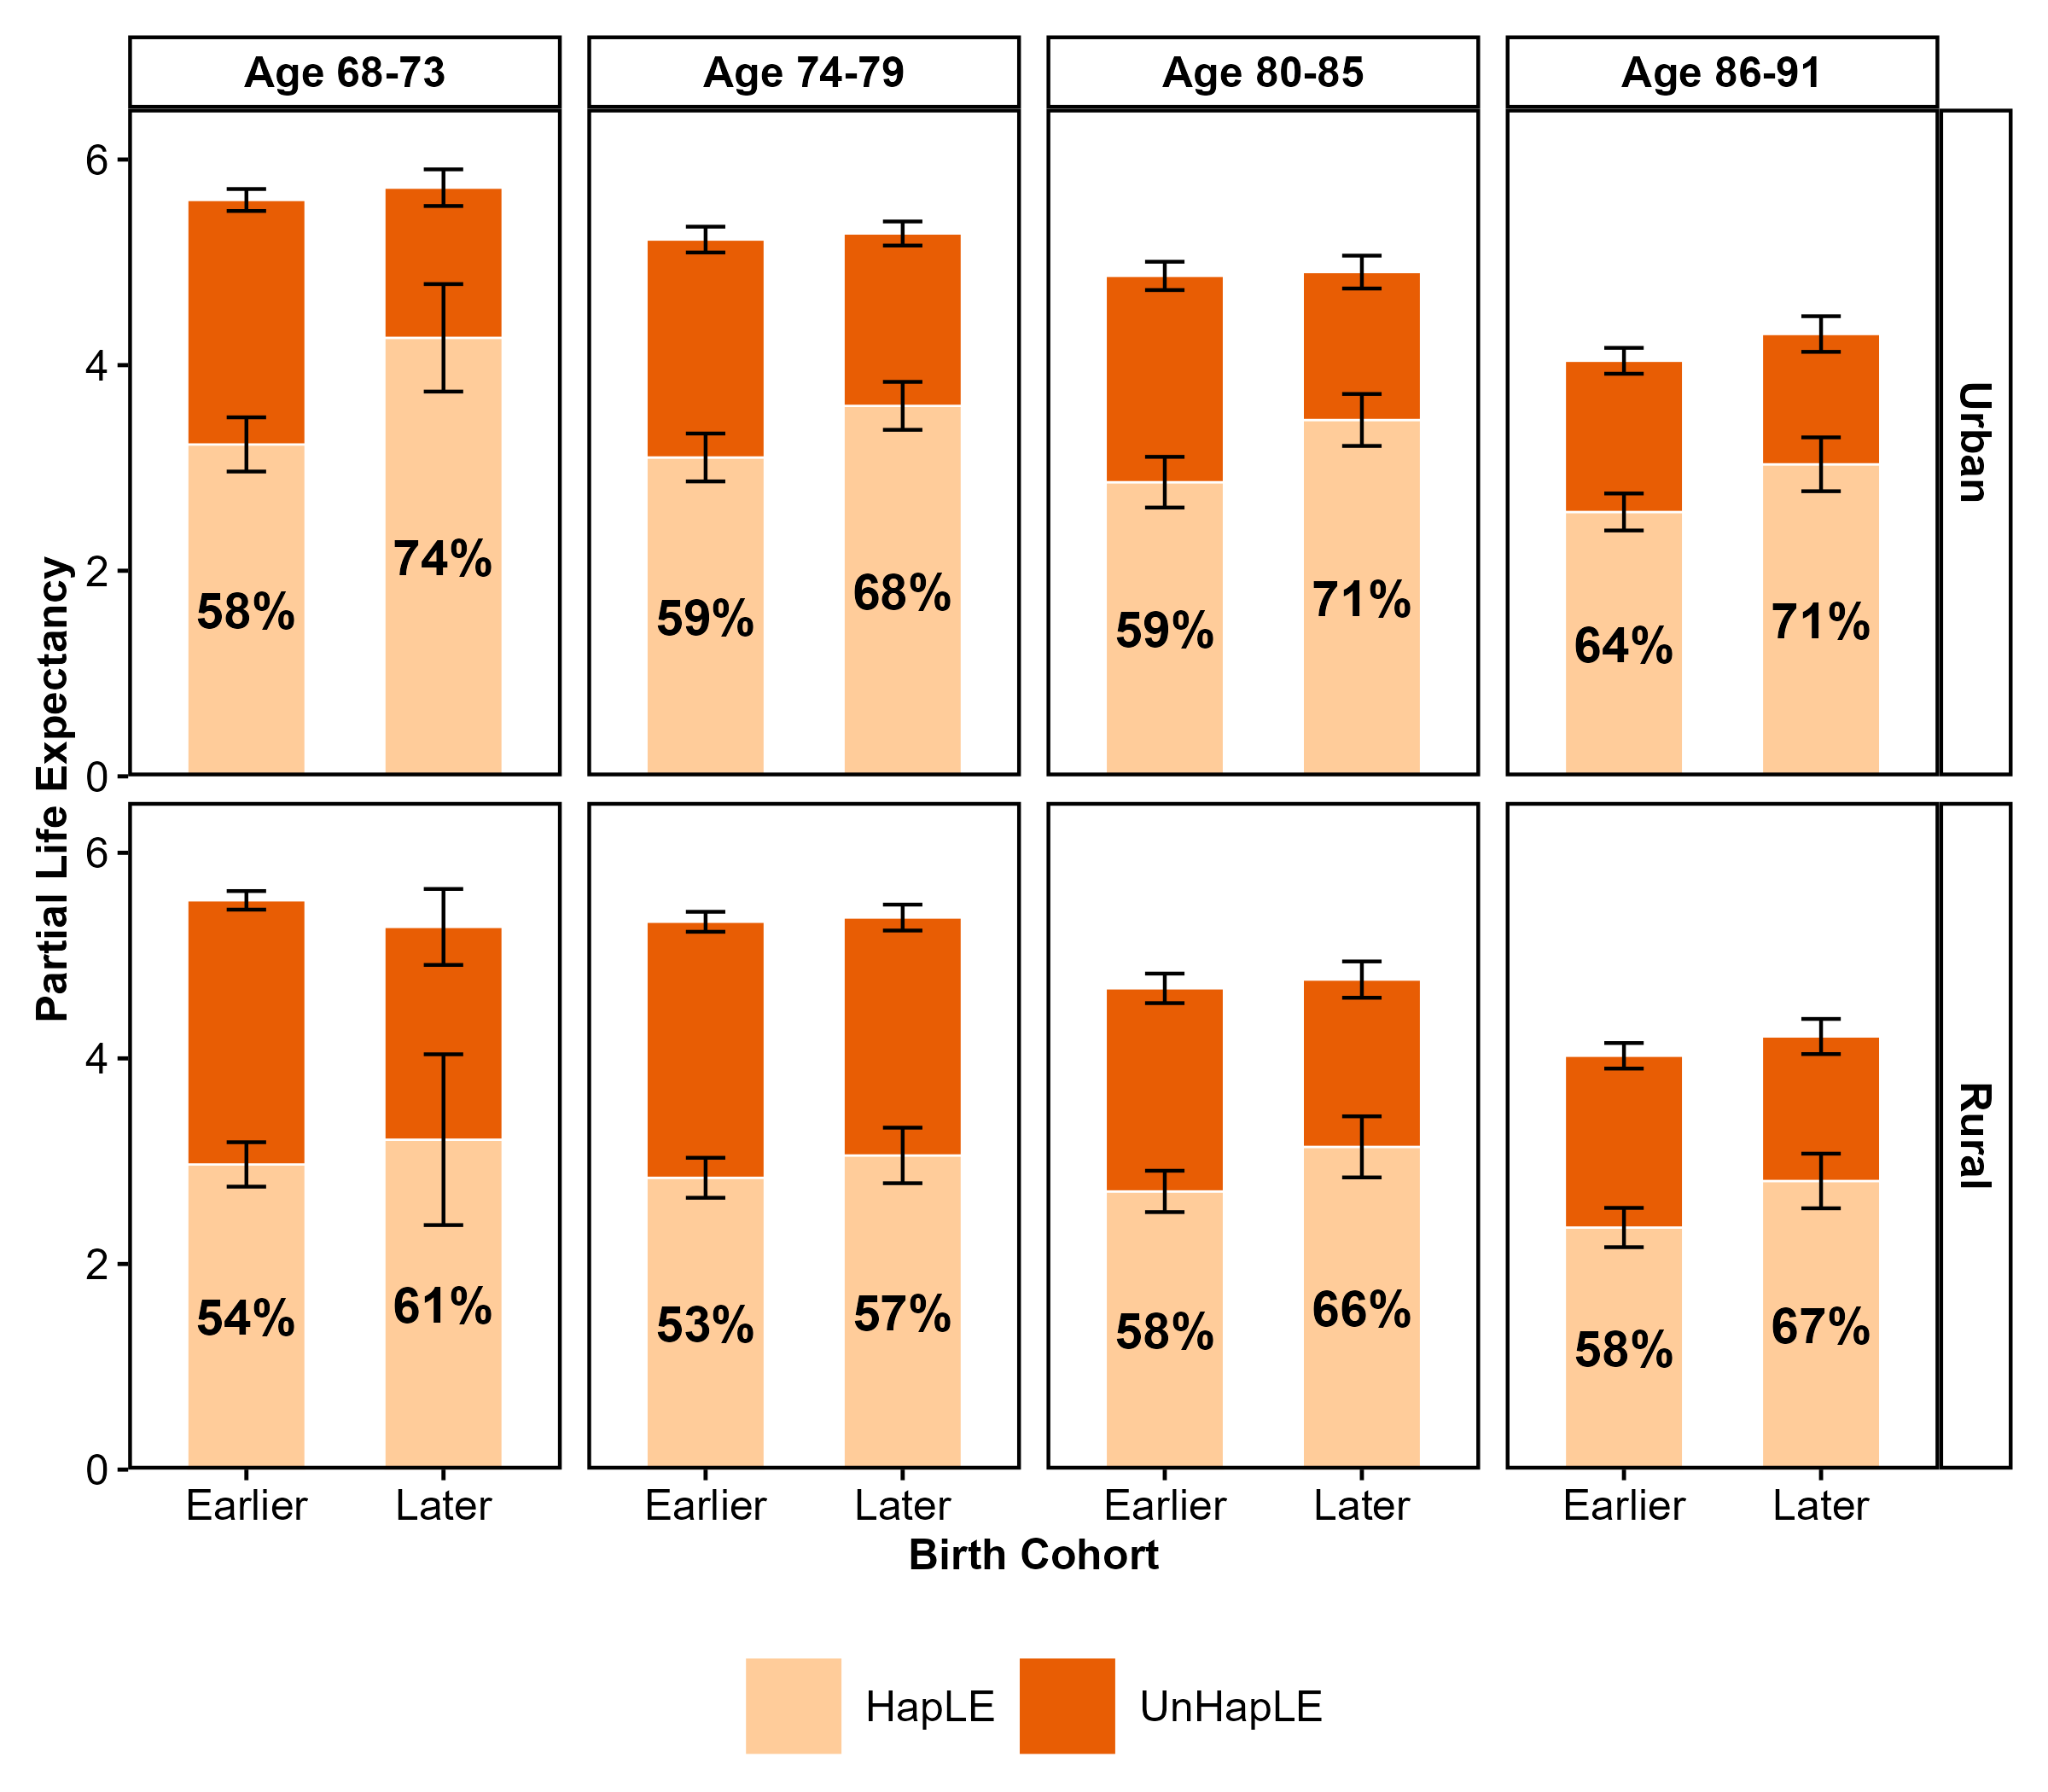
\includegraphics[width=1\textwidth]{fig_tabs_b300/2_4_HapLE_stacked_plots_urban.png}
  \caption{Estimated PC-LE, PC-HapLE and PC-UnHapLE by age range, birth cohorts and urban-rural residence. \textbf{Notes}: Each bar represents PC-LE for a specific birth cohort, age range, and residence. The bar is divided into PC-HapLE (light shading) and PC-UnHapLE (dark shading). The figure inside each bar indicates HapLE\%. Black vertical lines represent the 95\% CI for the PC-LE and PC-HapLE estimates. Values of estimates can also be found in Appendix Table S4. \textbf{Source}: Author's calculation based on CLHLS, 2002–2018.}
\end{figure}

%-------------------------------------------
% Discussion
%-------------------------------------------
\section{Discussion}

Using the national representative longitudinal data and a cohort-based multi-state life table approach, this study provides novel evidence to address the question of whether older adults in China are living longer happy years. Our findings reveal a significant and positive trend: later-born cohorts, across all examined age ranges from 68 to 91, are expected to live a greater number of years in a happy state and a higher proportion of their remaining life in happiness compared to their earlier-born counterparts. This gain in happy years was primarily achieved through a "compression of unhappiness"—a notable reduction in the expected years lived in an unhappy state—while total partial-cohort life expectancy remained largely stable across most age ranges. However, this optimistic aggregate trend masks profound and widening disparities. The gains in happy years were not equitably distributed, with improvements being substantially larger for women, literate individuals, and especially urban residents, suggesting that the benefits of socioeconomic progress have disproportionately favored more advantaged subgroups.

The observed "compression of unhappiness" across birth cohorts extends previous research and offers a cohort-based perspective on a widely debated topic in China. Our finding  is consistent with the period-based analysis by Duan and Chen \autocite{duan.2020.happy}, who also documented an "unhappiness compression" pattern in the general adult population. Our use of a cohort design provides stronger evidence that this is a generational phenomenon rather than a simple period effect \autocite{payne.2022.expansion}. This optimistic cohort trend also offers a nuanced counterpoint to the "Easterlin paradox," which posited that China’s rapid economic growth during the 1990s and early 2000s did not uniformly translate into greater life satisfaction \autocite{easterlin.2012.chinas,knight.2011.does,graham.2017.happiness}. Our results align more closely with recent studies indicating that Chinese happiness levels have been rising since the early 2000s, as the benefits of development became more widespread \autocite{wang.2023.hierarchical,cai.2023.does}. Several key factors likely contributed to the observed gains in happy life expectancy across the cohorts in our study. The observation periods of our analysis coincide with a period of maturation in China's social and economic systems. The older adults in our study were direct beneficiaries of the substantial expansion and consolidation of China's social security programs. The nationwide rollout of near-universal pension systems and health insurance schemes, including the New Rural Cooperative Medical System and the Urban Resident Basic Medical Insurance, provided a crucial buffer against economic and health-related shocks \autocite{liu.2019.are,guo.2024.regional,cheng.2021.sociodemographic}. This enhanced security, alongside improvements in public infrastructure \autocite{dong.2017.exploring} and the continued role of family support \autocite{zhao.2023.chinas,huang.2021.intergenerational}, has likely contributed to a more favorable environment for well-being in later life.

An interesting finding is the significant gender disparity in cohort differences, with older women experiencing substantially larger and more consistent gains in happy life expectancy (HapLE) than men. This finding contrasts with previous period-based evidence from China, which suggested that while women had a longer HapLE, this advantage was primarily driven by their lower mortality rather than a higher prevalence of happiness in later life \autocite{duan.2020.happy}. Our study reveals a fundamental shift: the gains in HapLE for women are driven by a “compression of unhappiness,” indicating an improvement in the quality, not just the quantity, of later-life years. One possible explanation for this phenomenon is that the trend is driven less by women’s objective conditions improving faster than men’s (the composition effect), and more by women deriving greater subjective well-being from the same life improvements (the coefficient effect) \autocite{yang.2024.gender}. Furthermore, women’s deeper embeddedness in family and community life means they likely gained more from improvements in community environments and social support systems, which are central to their daily routines and well-being \autocite{feng.2024.gender}.

Perhaps the most critical finding of this study is the widening socioeconomic gap in happy life expectancy, particularly between urban and rural residents. While previous research confirmed static inequalities at a single time point \autocite{wan.2024.socioeconomic}, our cohort analysis reveals a more troubling dynamic: the disparity is actively growing, creating a deepening "happiness gap." This growing urban-rural divide is likely rooted in China's dualistic socioeconomic structure, which has long favored urban areas in resource allocation. Urban older adults have consistently benefited from more generous pensions, higher-quality healthcare, and better-developed community infrastructure \autocite{liu.2019.are}. Although rural social security has improved, the level of protection remains substantially lower, leaving rural older adults less able to translate national development into personal well-being. Similarly, the education gap reflects disparities in the capacity to leverage resources. As a key determinant of socioeconomic status \autocite{link.1995.social, payne.2022.expansion,shen.2023.disability}, education equips individuals to better navigate complex healthcare and social welfare systems, an advantage that allows them to more effectively convert available opportunities into longer and happier lives \autocite{cheng.2021.sociodemographic,wan.2024.socioeconomic}. It is important to acknowledge that these two dimensions of inequality were analyzed in separate models due to the limitation of sample size. Given that urban populations in China are, on average, more educated, the effects we attribute to each factor are not fully disentangled. However, the fact that both show an independent predictive effect underscores that socioeconomic disadvantage is a multifaceted force. This suggests that while intertwined, the structural resource disparities and differences in individual capacity driving these gaps represent distinct mechanisms that warrant separate consideration.

Several limitations should be considered when interpreting the findings.First, our analysis is constrained by the measurement and classification of happiness. Our measurement of happiness relies on a single-item life satisfaction question, which, although widely validated and used in large-scale surveys, cannot capture the full multidimensional nature of well-being \autocite{george.2010.still}. Furthermore, our primary analysis dichotomizes responses into two states, which could be viewed as subjective. To test the robustness of this classification, we conducted a sensitivity analysis using a four-state model and the results strongly corroborate our main conclusions. Second, our model specification was limited by sample size. We did not control potential confounders such as health status. Similarly, we analyzed education and residence in separate models and could not explore their interaction. Future research with larger datasets is needed to disentangle these complex relationships. Third, our analysis focuses on life expectancies within bounded age ranges rather than complete life-course measures. While this approach enables the examination of living cohorts, the results should not be directly extrapolated to full lifetime happiness trajectories, particularly given the potential for major social or policy disruptions that could alter later-life patterns \autocite{payne.2022.expansion}. Fourth, the multistate life table model employed in this study is based on a first-order Markov assumption, meaning that happiness transitions depend only on the current state and not on the duration spent in that state or past emotional trajectories \autocite{payne.2022.expansion,shen.2023.disability}. This simplifies the complex psychological dynamics of well-being in reality. Related to this, the panel nature of CLHLS data, with surveys conducted every three or four years, assumes only annual transitions between waves, potentially missing short-term fluctuations or multiple transitions in happiness states that may occur between survey periods. However, prior work suggests such limitations may not severely compromise the overall life expectancy estimates \autocite{liu.2019.are}.

One of the main strengths of this study is its focus on understanding changes in happy life expectancy across birth cohorts, rather than relying solely on period-based comparisons. Though period-based approach may be useful for monitoring aggregate trends in population-level happiness, these results do not easily translate to the experience of any given cohort of individuals \autocite{payne.2022.expansion}. Our cohort-based approach provides results that match more closely with the lived experience of individuals within the population and offers clearer insights into generational changes in happy longevity. A second strength lies in our comprehensive examination of socioeconomic disparities in HapLE trends. While previous studies have documented static inequalities in HapLE at single time points \autocite{wan.2024.socioeconomic}, our analysis reveals the dynamic patterns of how these disparities evolve across cohorts, thus providing new evidence on whether the benefits of China's socioeconomic development are being equitably distributed across different population subgroups. Additionally, our analysis uses CLHLS, one of the largest and most comprehensive longitudinal datasets of older adults worldwide, providing a unique opportunity to examine happiness trajectories among a substantial portion of the global aging population. The combination of this data source with the multistate life table method enables robust estimation of HapLE across cohorts and subgroups, supporting the reliability and generalizability of our findings.
%-------------------------------------------
% Conclusion
%-------------------------------------------
\section{Conclusion}

In conclusion, this study provides evidence that older adults in China are indeed living longer happy years across birth cohorts, largely driven by a significant "compression of unhappiness" rather than an extension of total lifespan. This optimistic aggregate trend, however, conceals a crucial and troubling counter-narrative: the profound widening of a "happiness gap." The benefits of China's rapid socioeconomic development have not been equitably distributed, disproportionately favoring urban, educated, and female older adults. While these advantaged groups are experiencing accelerated gains in happiness, their rural and less-educated counterparts are being left behind, creating a deepening divide in the quality of later life. These findings challenge policymakers to look beyond extending longevity and to urgently address the structural inequalities that prevent the gains of national progress from translating into universal well-being. To foster a truly equitable aging society, future policy must pivot from simply adding years to life, to ensuring that those added years are happy ones for all.

%-------------------------------------------
% References
%-------------------------------------------
\newpage
\printbibliography

%-------------------------------------------
% Appendix
%-------------------------------------------
\renewcommand\theequation{\Alph{section}\arabic{equation}} %Redefine equation numbering format
\counterwithin*{equation}{section} % Number equations within sections
\renewcommand\thefigure{\Alph{section}\arabic{figure}} % Redefine equation numbering format
\counterwithin*{figure}{section} % Number equations within sections
% Manual table numbering for supplementary tables (S1, S2, S3, S4)

\newpage
\begin{appendices}

  \section*{Appendix}

  % === Figure S1 ===
  \begin{figure}[htbp]
    \centering
    \caption*{\textbf{Figure S1.} State space in the 4-state model}
    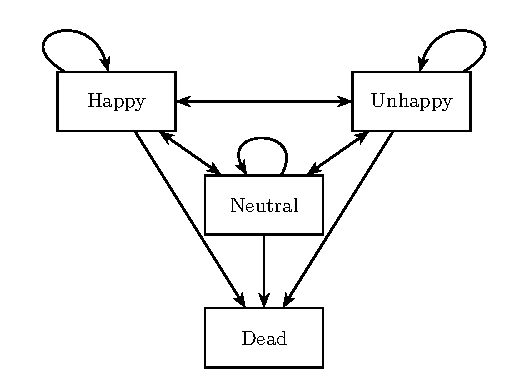
\includegraphics[width=0.8\textwidth]{fig_tabs_b300/latex_output/State_space_4s.pdf}
    \label{fig:State_space_4s}
  \end{figure}


  % === Table S1: Descriptive Table ===
  \vspace*{\fill}
  \begin{table}[!h]
    \centering
    \caption*{\textbf{Table S1.} Baseline characteristics of study participants by age range and birth cohort}
    \label{tab:S1_desc_stats}
    \resizebox{\ifdim\width>\linewidth\linewidth\else\width\fi}{!}{%
      \begin{tabular}{lcccccccc}
        \toprule
        \textbf{Age Range} & \multicolumn{2}{c}{\textbf{68--73}} & \multicolumn{2}{c}{\textbf{74--79}} & \multicolumn{2}{c}{\textbf{80--85}} & \multicolumn{2}{c}{\textbf{86--91}}                                                                                 \\
        \cmidrule(lr){2-3} \cmidrule(lr){4-5} \cmidrule(lr){6-7} \cmidrule(lr){8-9}
        \textbf{Cohort}    & \textbf{1932--37}                   & \textbf{1942--47}                   & \textbf{1926--31}                   & \textbf{1936--41}                   & \textbf{1920--25} & \textbf{1930--35} & \textbf{1914--19} & \textbf{1924--29} \\
        \midrule
        \textbf{N}         & 1643                                & 754                                 & 1677                                & 1370                                & 1764              & 1200              & 2191              & 1435              \\
        \midrule
        \textbf{Gender (\%)}                                                                                                                                                                                                                                       \\
        \quad Men          & 51.7                                & 56.0                                & 50.4                                & 53.2                                & 51.4              & 51.6              & 50.6              & 51.5              \\
        \quad Women        & 48.3                                & 44.0                                & 49.6                                & 46.8                                & 48.6              & 48.4              & 49.4              & 48.5              \\
        \midrule
        \textbf{Education (\%)}                                                                                                                                                                                                                                    \\
        \quad Literate     & 57.6                                & 72.7                                & 49.3                                & 60.2                                & 43.7              & 48.0              & 43.3              & 40.1              \\
        \quad Illiterate   & 42.4                                & 27.3                                & 50.7                                & 39.8                                & 56.3              & 52.0              & 56.7              & 59.9              \\
        \midrule
        \textbf{Residence (\%)}                                                                                                                                                                                                                                    \\
        \quad Urban        & 41.3                                & 41.9                                & 40.9                                & 51.0                                & 43.4              & 50.0              & 49.9              & 48.2              \\
        \quad Rural        & 58.7                                & 58.1                                & 59.1                                & 49.0                                & 56.6              & 50.0              & 50.1              & 51.8              \\
        \midrule
        \textbf{Happiness (3-state model) (\%)}                                                                                                                                                                                                                    \\
        \quad Happy        & 56.7                                & 58.6                                & 57.1                                & 56.9                                & 58.4              & 60.2              & 58.6              & 57.7              \\
        \quad Unhappy      & 43.3                                & 41.4                                & 42.9                                & 43.1                                & 41.6              & 39.8              & 41.4              & 42.3              \\
        \midrule
        \textbf{Happiness (4-state model) (\%)}                                                                                                                                                                                                                    \\
        \quad Happy        & 56.7                                & 58.6                                & 57.1                                & 56.9                                & 58.4              & 60.2              & 58.6              & 57.7              \\
        \quad Neutral      & 36.6                                & 37.9                                & 36.3                                & 37.2                                & 33.8              & 33.9              & 33.2              & 35.0              \\
        \quad Unhappy      & 6.7                                 & 3.4                                 & 6.6                                 & 5.9                                 & 7.7               & 5.9               & 8.2               & 7.3               \\
        \midrule
        \textbf{Disability (\%)}                                                                                                                                                                                                                                   \\
        \quad 0 ADL        & 96.3                                & 95.8                                & 93.4                                & 92.8                                & 86.2              & 88.4              & 76.6              & 81.6              \\
        \quad 1+ ADL       & 3.7                                 & 4.2                                 & 6.6                                 & 7.2                                 & 13.8              & 11.6              & 23.4              & 18.4              \\
        \bottomrule
      \end{tabular}%
    }
  \end{table}
  \vspace*{\fill}

  % === Table S2 ===
  \vspace*{\fill}
  \begin{table}[!p]
    \centering
    \caption*{\textbf{Table S2.} Estimated PC-LE, PC-HapLE, PC-UnHapLE, HapLE\% and UnHapLE\% and cohort differences, by age range and sex. \textbf{Notes}: The \textit{Diff.} row represents the difference calculated as the later cohort's value minus the earlier cohort's value. Values in parentheses are 95\% CI. Significance of the difference is denoted by: * p$<$0.05, ** p$<$0.01, *** p$<$0.001. \textbf{Source}: Author's calculation based on CLHLS, 2002–2018.}
    \centering
    \resizebox{\ifdim\width>\linewidth\linewidth\else\width\fi}{!}{
      \begin{tabular}[t]{>{}l>{}lllllll}
        \toprule
        \textbf{Age Range}                    & \textbf{Sex}                      & \textbf{Cohort}               & \textbf{PC-LE}                              & \textbf{PC-HapLE}                            & \textbf{HapLE\%}                            & \textbf{PC-UnHapLE}                             & \textbf{UnHapLE\%}                             \\
        \midrule
        \multirow{9}{*}[-4ex]{\textbf{68-73}} & \multirow{3}{*}{\textbf{Overall}} & Earlier                       & 5.56 (5.49, 5.63)                           & 3.07 (2.91, 3.23)                            & 55.2 (52.3, 58.1)                           & 2.49 (2.33, 2.66)                               & 44.8 (41.9, 47.7)                              \\
        \cmidrule{3-8}
                                              &                                   & Later                         & 5.50 (5.27, 5.74)                           & 3.67 (3.09, 4.25)                            & 66.7 (57.6, 75.9)                           & 1.83 (1.35, 2.31)                               & 33.3 (24.1, 42.4)                              \\
        \cmidrule{3-8}
                                              &                                   & \cellcolor{gray!10}\em{Diff.} & \cellcolor{gray!10}\em{-0.06 (-0.30, 0.19)} & \cellcolor{gray!10}\em{0.60 (0.00, 1.21)*}   & \cellcolor{gray!10}\em{11.5 (2.0, 21.1)*}   & \cellcolor{gray!10}\em{-0.66 (-1.17, -0.16)*}   & \cellcolor{gray!10}\em{-11.5 (-21.1, -2.0)*}   \\
        \cmidrule{2-8}
                                              & \multirow{3}{*}{\textbf{Men}}     & Earlier                       & 5.51 (5.42, 5.61)                           & 3.02 (2.80, 3.25)                            & 54.8 (50.9, 58.8)                           & 2.49 (2.27, 2.71)                               & 45.2 (41.2, 49.1)                              \\
        \cmidrule{3-8}
                                              &                                   & Later                         & 5.37 (5.03, 5.71)                           & 3.36 (2.65, 4.07)                            & 62.5 (51.1, 74.0)                           & 2.01 (1.42, 2.60)                               & 37.5 (26.0, 48.9)                              \\
        \cmidrule{3-8}
                                              &                                   & \cellcolor{gray!10}\em{Diff.} & \cellcolor{gray!10}\em{-0.15 (-0.50, 0.21)} & \cellcolor{gray!10}\em{0.34 (-0.41, 1.08)}   & \cellcolor{gray!10}\em{7.7 (-4.4, 19.9)}    & \cellcolor{gray!10}\em{-0.48 (-1.11, 0.15)}     & \cellcolor{gray!10}\em{-7.7 (-19.9, 4.4)}      \\
        \cmidrule{2-8}
                                              & \multirow{3}{*}{\textbf{Women}}   & Earlier                       & 5.60 (5.51, 5.69)                           & 3.11 (2.88, 3.35)                            & 55.6 (51.4, 59.7)                           & 2.49 (2.25, 2.73)                               & 44.4 (40.3, 48.6)                              \\
        \cmidrule{3-8}
                                              &                                   & Later                         & 5.66 (5.39, 5.93)                           & 4.01 (3.27, 4.75)                            & 70.9 (59.5, 82.3)                           & 1.65 (1.04, 2.26)                               & 29.1 (17.7, 40.5)                              \\
        \cmidrule{3-8}
                                              &                                   & \cellcolor{gray!10}\em{Diff.} & \cellcolor{gray!10}\em{0.06 (-0.22, 0.34)}  & \cellcolor{gray!10}\em{0.90 (0.12, 1.68)*}   & \cellcolor{gray!10}\em{15.3 (3.2, 27.4)*}   & \cellcolor{gray!10}\em{-0.84 (-1.50, -0.18)*}   & \cellcolor{gray!10}\em{-15.3 (-27.4, -3.2)*}   \\
        \cmidrule{1-8}
        \multirow{9}{*}[-4ex]{\textbf{74-79}} & \multirow{3}{*}{\textbf{Overall}} & Earlier                       & 5.30 (5.22, 5.38)                           & 2.93 (2.77, 3.09)                            & 55.3 (52.5, 58.2)                           & 2.37 (2.22, 2.52)                               & 44.7 (41.8, 47.5)                              \\
        \cmidrule{3-8}
                                              &                                   & Later                         & 5.33 (5.24, 5.43)                           & 3.32 (3.12, 3.52)                            & 62.3 (58.7, 65.9)                           & 2.01 (1.81, 2.21)                               & 37.7 (34.1, 41.3)                              \\
        \cmidrule{3-8}
                                              &                                   & \cellcolor{gray!10}\em{Diff.} & \cellcolor{gray!10}\em{0.04 (-0.08, 0.16)}  & \cellcolor{gray!10}\em{0.39 (0.14, 0.65)**}  & \cellcolor{gray!10}\em{7.0 (2.4, 11.6)**}   & \cellcolor{gray!10}\em{-0.36 (-0.61, -0.11)**}  & \cellcolor{gray!10}\em{-7.0 (-11.6, -2.4)**}   \\
        \cmidrule{2-8}
                                              & \multirow{3}{*}{\textbf{Men}}     & Earlier                       & 5.23 (5.12, 5.34)                           & 3.03 (2.82, 3.24)                            & 57.9 (54.2, 61.6)                           & 2.20 (2.01, 2.40)                               & 42.1 (38.4, 45.8)                              \\
        \cmidrule{3-8}
                                              &                                   & Later                         & 5.14 (5.00, 5.29)                           & 3.13 (2.88, 3.37)                            & 60.8 (56.3, 65.3)                           & 2.02 (1.78, 2.26)                               & 39.2 (34.7, 43.7)                              \\
        \cmidrule{3-8}
                                              &                                   & \cellcolor{gray!10}\em{Diff.} & \cellcolor{gray!10}\em{-0.08 (-0.26, 0.09)} & \cellcolor{gray!10}\em{0.10 (-0.22, 0.42)}   & \cellcolor{gray!10}\em{2.9 (-3.0, 8.7)}     & \cellcolor{gray!10}\em{-0.18 (-0.49, 0.13)}     & \cellcolor{gray!10}\em{-2.9 (-8.7, 3.0)}       \\
        \cmidrule{2-8}
                                              & \multirow{3}{*}{\textbf{Women}}   & Earlier                       & 5.36 (5.26, 5.46)                           & 2.84 (2.63, 3.06)                            & 53.1 (49.1, 57.0)                           & 2.52 (2.30, 2.73)                               & 46.9 (43.0, 50.9)                              \\
        \cmidrule{3-8}
                                              &                                   & Later                         & 5.52 (5.43, 5.62)                           & 3.48 (3.21, 3.75)                            & 63.0 (58.2, 67.8)                           & 2.04 (1.77, 2.31)                               & 37.0 (32.2, 41.8)                              \\
        \cmidrule{3-8}
                                              &                                   & \cellcolor{gray!10}\em{Diff.} & \cellcolor{gray!10}\em{0.16 (0.02, 0.30)*}  & \cellcolor{gray!10}\em{0.64 (0.29, 0.99)***} & \cellcolor{gray!10}\em{10.0 (3.8, 16.2)***} & \cellcolor{gray!10}\em{-0.47 (-0.82, -0.13)**}  & \cellcolor{gray!10}\em{-10.0 (-16.2, -3.8)**}  \\
        \cmidrule{1-8}
        \multirow{9}{*}[-4ex]{\textbf{80-85}} & \multirow{3}{*}{\textbf{Overall}} & Earlier                       & 4.74 (4.63, 4.85)                           & 2.75 (2.58, 2.92)                            & 58.0 (54.8, 61.2)                           & 1.99 (1.83, 2.15)                               & 42.0 (38.8, 45.2)                              \\
        \cmidrule{3-8}
                                              &                                   & Later                         & 4.84 (4.71, 4.97)                           & 3.29 (3.08, 3.51)                            & 68.1 (64.3, 71.9)                           & 1.54 (1.36, 1.72)                               & 31.9 (28.1, 35.7)                              \\
        \cmidrule{3-8}
                                              &                                   & \cellcolor{gray!10}\em{Diff.} & \cellcolor{gray!10}\em{0.10 (-0.07, 0.27)}  & \cellcolor{gray!10}\em{0.55 (0.27, 0.82)***} & \cellcolor{gray!10}\em{10.1 (5.1, 15.1)***} & \cellcolor{gray!10}\em{-0.45 (-0.69, -0.21)***} & \cellcolor{gray!10}\em{-10.1 (-15.1, -5.1)***} \\
        \cmidrule{2-8}
                                              & \multirow{3}{*}{\textbf{Men}}     & Earlier                       & 4.60 (4.46, 4.74)                           & 2.74 (2.51, 2.97)                            & 59.5 (55.0, 64.1)                           & 1.86 (1.65, 2.08)                               & 40.5 (35.9, 45.0)                              \\
        \cmidrule{3-8}
                                              &                                   & Later                         & 4.70 (4.52, 4.88)                           & 3.09 (2.82, 3.36)                            & 65.8 (60.8, 70.8)                           & 1.61 (1.36, 1.85)                               & 34.2 (29.2, 39.2)                              \\
        \cmidrule{3-8}
                                              &                                   & \cellcolor{gray!10}\em{Diff.} & \cellcolor{gray!10}\em{0.10 (-0.13, 0.33)}  & \cellcolor{gray!10}\em{0.35 (0.00, 0.70)*}   & \cellcolor{gray!10}\em{6.3 (-0.5, 13.0)}    & \cellcolor{gray!10}\em{-0.25 (-0.58, 0.07)}     & \cellcolor{gray!10}\em{-6.3 (-13.0, 0.5)}      \\
        \cmidrule{2-8}
                                              & \multirow{3}{*}{\textbf{Women}}   & Earlier                       & 4.85 (4.71, 5.00)                           & 2.76 (2.54, 2.98)                            & 56.9 (52.7, 61.0)                           & 2.09 (1.88, 2.30)                               & 43.1 (39.0, 47.3)                              \\
        \cmidrule{3-8}
                                              &                                   & Later                         & 4.95 (4.77, 5.12)                           & 3.44 (3.15, 3.73)                            & 69.6 (64.6, 74.5)                           & 1.51 (1.27, 1.74)                               & 30.4 (25.5, 35.4)                              \\
        \cmidrule{3-8}
                                              &                                   & \cellcolor{gray!10}\em{Diff.} & \cellcolor{gray!10}\em{0.09 (-0.13, 0.32)}  & \cellcolor{gray!10}\em{0.68 (0.31, 1.05)***} & \cellcolor{gray!10}\em{12.7 (6.2, 19.2)***} & \cellcolor{gray!10}\em{-0.59 (-0.91, -0.27)***} & \cellcolor{gray!10}\em{-12.7 (-19.2, -6.2)***} \\
        \cmidrule{1-8}
        \multirow{9}{*}[-4ex]{\textbf{86-91}} & \multirow{3}{*}{\textbf{Overall}} & Earlier                       & 4.03 (3.93, 4.13)                           & 2.43 (2.28, 2.57)                            & 60.2 (57.0, 63.4)                           & 1.61 (1.47, 1.74)                               & 39.8 (36.6, 43.0)                              \\
        \cmidrule{3-8}
                                              &                                   & Later                         & 4.25 (4.11, 4.38)                           & 2.90 (2.71, 3.10)                            & 68.4 (64.6, 72.2)                           & 1.34 (1.18, 1.50)                               & 31.6 (27.8, 35.4)                              \\
        \cmidrule{3-8}
                                              &                                   & \cellcolor{gray!10}\em{Diff.} & \cellcolor{gray!10}\em{0.21 (0.05, 0.38)*}  & \cellcolor{gray!10}\em{0.48 (0.23, 0.72)***} & \cellcolor{gray!10}\em{8.2 (3.2, 13.2)**}   & \cellcolor{gray!10}\em{-0.26 (-0.47, -0.05)*}   & \cellcolor{gray!10}\em{-8.2 (-13.2, -3.2)**}   \\
        \cmidrule{2-8}
                                              & \multirow{3}{*}{\textbf{Men}}     & Earlier                       & 3.79 (3.67, 3.92)                           & 2.30 (2.12, 2.48)                            & 60.6 (56.2, 64.9)                           & 1.50 (1.32, 1.67)                               & 39.4 (35.1, 43.8)                              \\
        \cmidrule{3-8}
                                              &                                   & Later                         & 3.99 (3.81, 4.17)                           & 2.73 (2.49, 2.96)                            & 68.3 (63.5, 73.1)                           & 1.27 (1.07, 1.46)                               & 31.7 (26.9, 36.5)                              \\
        \cmidrule{3-8}
                                              &                                   & \cellcolor{gray!10}\em{Diff.} & \cellcolor{gray!10}\em{0.20 (-0.02, 0.42)}  & \cellcolor{gray!10}\em{0.43 (0.13, 0.73)**}  & \cellcolor{gray!10}\em{7.7 (1.2, 14.2)*}    & \cellcolor{gray!10}\em{-0.23 (-0.49, 0.03)}     & \cellcolor{gray!10}\em{-7.7 (-14.2, -1.2)*}    \\
        \cmidrule{2-8}
                                              & \multirow{3}{*}{\textbf{Women}}   & Earlier                       & 4.17 (4.05, 4.30)                           & 2.49 (2.29, 2.69)                            & 59.6 (55.3, 63.9)                           & 1.68 (1.50, 1.87)                               & 40.4 (36.1, 44.7)                              \\
        \cmidrule{3-8}
                                              &                                   & Later                         & 4.39 (4.23, 4.56)                           & 3.01 (2.75, 3.26)                            & 68.4 (63.3, 73.5)                           & 1.39 (1.16, 1.61)                               & 31.6 (26.5, 36.7)                              \\
        \cmidrule{3-8}
                                              &                                   & \cellcolor{gray!10}\em{Diff.} & \cellcolor{gray!10}\em{0.22 (0.01, 0.43)*}  & \cellcolor{gray!10}\em{0.52 (0.19, 0.84)**}  & \cellcolor{gray!10}\em{8.8 (2.1, 15.4)**}   & \cellcolor{gray!10}\em{-0.30 (-0.58, -0.01)*}   & \cellcolor{gray!10}\em{-8.8 (-15.4, -2.1)**}   \\
        \bottomrule
      \end{tabular}}
  \end{table}
  \vspace*{\fill}

  % === Table S3 ===
  \vspace*{\fill}
  \begin{table}[!p]
    \centering
    \caption*{\textbf{Table S3.} Estimated PC-LE, PC-HapLE, PC-UnHapLE, HapLE\% and UnHapLE\% and cohort differences, by age range and education level. \textbf{Notes}: The \textit{Diff.} row represents the difference calculated as the later cohort's value minus the earlier cohort's value. Values in parentheses are 95\% CI. Significance of the difference is denoted by: * p$<$0.05, ** p$<$0.01, *** p$<$0.001. \textbf{Source}: Author's calculation based on CLHLS, 2002–2018.}
    \centering
    \resizebox{\ifdim\width>\linewidth\linewidth\else\width\fi}{!}{
      \begin{tabular}[t]{>{}l>{}lllllll}
        \toprule
        \textbf{Age Range}                    & \textbf{Education}                   & \textbf{Cohort}               & \textbf{PC-LE}                              & \textbf{PC-HapLE}                           & \textbf{HapLE\%}                            & \textbf{PC-UnHapLE}                             & \textbf{UnHapLE\%}                             \\
        \midrule
        \multirow{9}{*}[-0ex]{\textbf{68-73}} & \multirow{3}{*}{\textbf{Literate}}   & Earlier                       & 5.60 (5.51, 5.68)                           & 3.23 (3.01, 3.44)                           & 57.7 (54.0, 61.4)                           & 2.37 (2.16, 2.58)                               & 42.3 (38.6, 46.0)                              \\
        \cmidrule{3-8}
                                              &                                      & Later                         & 5.52 (5.25, 5.79)                           & 3.80 (3.23, 4.36)                           & 68.8 (59.8, 77.8)                           & 1.72 (1.24, 2.21)                               & 31.2 (22.2, 40.2)                              \\
        \cmidrule{3-8}
                                              &                                      & \cellcolor{gray!10}\em{Diff.} & \cellcolor{gray!10}\em{-0.08 (-0.36, 0.20)} & \cellcolor{gray!10}\em{0.57 (-0.03, 1.17)}  & \cellcolor{gray!10}\em{11.1 (1.4, 20.8)*}   & \cellcolor{gray!10}\em{-0.65 (-1.17, -0.12)*}   & \cellcolor{gray!10}\em{-11.1 (-20.8, -1.4)*}   \\
        \cmidrule{2-8}
                                              & \multirow{3}{*}{\textbf{Illiterate}} & Earlier                       & 5.45 (5.30, 5.61)                           & 2.85 (2.55, 3.14)                           & 52.2 (46.9, 57.4)                           & 2.61 (2.31, 2.91)                               & 47.8 (42.6, 53.1)                              \\
        \cmidrule{3-8}
                                              &                                      & Later                         & 5.32 (4.92, 5.73)                           & 3.28 (2.24, 4.31)                           & 61.6 (45.6, 77.6)                           & 2.05 (1.28, 2.81)                               & 38.4 (22.4, 54.4)                              \\
        \cmidrule{3-8}
                                              &                                      & \cellcolor{gray!10}\em{Diff.} & \cellcolor{gray!10}\em{-0.13 (-0.57, 0.30)} & \cellcolor{gray!10}\em{0.43 (-0.65, 1.51)}  & \cellcolor{gray!10}\em{9.4 (-7.5, 26.2)}    & \cellcolor{gray!10}\em{-0.56 (-1.38, 0.26)}     & \cellcolor{gray!10}\em{-9.4 (-26.2, 7.5)}      \\
        \cmidrule{1-8}
        \multirow{9}{*}[-0ex]{\textbf{74-79}} & \multirow{3}{*}{\textbf{Literate}}   & Earlier                       & 5.34 (5.22, 5.45)                           & 3.00 (2.77, 3.23)                           & 56.3 (52.2, 60.4)                           & 2.33 (2.11, 2.56)                               & 43.7 (39.6, 47.8)                              \\
        \cmidrule{3-8}
                                              &                                      & Later                         & 5.36 (5.25, 5.47)                           & 3.47 (3.20, 3.74)                           & 64.7 (59.9, 69.5)                           & 1.89 (1.63, 2.15)                               & 35.3 (30.5, 40.1)                              \\
        \cmidrule{3-8}
                                              &                                      & \cellcolor{gray!10}\em{Diff.} & \cellcolor{gray!10}\em{0.02 (-0.13, 0.18)}  & \cellcolor{gray!10}\em{0.47 (0.11, 0.82)**} & \cellcolor{gray!10}\em{8.5 (2.2, 14.8)**}   & \cellcolor{gray!10}\em{-0.44 (-0.78, -0.10)*}   & \cellcolor{gray!10}\em{-8.5 (-14.8, -2.2)**}   \\
        \cmidrule{2-8}
                                              & \multirow{3}{*}{\textbf{Illiterate}} & Earlier                       & 5.28 (5.16, 5.40)                           & 2.78 (2.55, 3.01)                           & 52.6 (48.5, 56.8)                           & 2.50 (2.28, 2.72)                               & 47.4 (43.2, 51.5)                              \\
        \cmidrule{3-8}
                                              &                                      & Later                         & 5.31 (5.16, 5.46)                           & 2.96 (2.66, 3.26)                           & 55.8 (50.1, 61.5)                           & 2.35 (2.03, 2.67)                               & 44.2 (38.5, 49.9)                              \\
        \cmidrule{3-8}
                                              &                                      & \cellcolor{gray!10}\em{Diff.} & \cellcolor{gray!10}\em{0.03 (-0.16, 0.22)}  & \cellcolor{gray!10}\em{0.18 (-0.20, 0.56)}  & \cellcolor{gray!10}\em{3.1 (-3.9, 10.2)}    & \cellcolor{gray!10}\em{-0.15 (-0.54, 0.23)}     & \cellcolor{gray!10}\em{-3.1 (-10.2, 3.9)}      \\
        \cmidrule{1-8}
        \multirow{9}{*}[-0ex]{\textbf{80-85}} & \multirow{3}{*}{\textbf{Literate}}   & Earlier                       & 4.81 (4.62, 5.00)                           & 2.74 (2.45, 3.03)                           & 57.0 (51.1, 62.8)                           & 2.07 (1.77, 2.37)                               & 43.0 (37.2, 48.9)                              \\
        \cmidrule{3-8}
                                              &                                      & Later                         & 4.85 (4.65, 5.04)                           & 3.46 (3.14, 3.78)                           & 71.3 (65.8, 76.8)                           & 1.39 (1.13, 1.65)                               & 28.7 (23.2, 34.2)                              \\
        \cmidrule{3-8}
                                              &                                      & \cellcolor{gray!10}\em{Diff.} & \cellcolor{gray!10}\em{0.04 (-0.23, 0.31)}  & \cellcolor{gray!10}\em{0.72 (0.28, 1.15)**} & \cellcolor{gray!10}\em{14.4 (6.3, 22.4)***} & \cellcolor{gray!10}\em{-0.68 (-1.08, -0.28)***} & \cellcolor{gray!10}\em{-14.4 (-22.4, -6.3)***} \\
        \cmidrule{2-8}
                                              & \multirow{3}{*}{\textbf{Illiterate}} & Earlier                       & 4.72 (4.58, 4.86)                           & 2.78 (2.56, 3.01)                           & 59.0 (54.8, 63.2)                           & 1.93 (1.73, 2.13)                               & 41.0 (36.8, 45.2)                              \\
        \cmidrule{3-8}
                                              &                                      & Later                         & 4.84 (4.66, 5.03)                           & 3.19 (2.89, 3.48)                           & 65.8 (60.6, 70.9)                           & 1.66 (1.41, 1.90)                               & 34.2 (29.1, 39.4)                              \\
        \cmidrule{3-8}
                                              &                                      & \cellcolor{gray!10}\em{Diff.} & \cellcolor{gray!10}\em{0.12 (-0.11, 0.36)}  & \cellcolor{gray!10}\em{0.40 (0.03, 0.77)*}  & \cellcolor{gray!10}\em{6.8 (0.1, 13.4)*}    & \cellcolor{gray!10}\em{-0.28 (-0.60, 0.04)}     & \cellcolor{gray!10}\em{-6.8 (-13.4, -0.1)*}    \\
        \cmidrule{1-8}
        \multirow{9}{*}[-0ex]{\textbf{86-91}} & \multirow{3}{*}{\textbf{Literate}}   & Earlier                       & 4.00 (3.80, 4.20)                           & 2.43 (2.14, 2.72)                           & 60.8 (54.3, 67.4)                           & 1.57 (1.29, 1.84)                               & 39.2 (32.6, 45.7)                              \\
        \cmidrule{3-8}
                                              &                                      & Later                         & 4.50 (4.28, 4.72)                           & 3.14 (2.76, 3.52)                           & 69.9 (62.7, 77.0)                           & 1.35 (1.04, 1.67)                               & 30.1 (23.0, 37.3)                              \\
        \cmidrule{3-8}
                                              &                                      & \cellcolor{gray!10}\em{Diff.} & \cellcolor{gray!10}\em{0.50 (0.20, 0.79)**} & \cellcolor{gray!10}\em{0.71 (0.23, 1.19)**} & \cellcolor{gray!10}\em{9.0 (-0.7, 18.8)}    & \cellcolor{gray!10}\em{-0.21 (-0.63, 0.20)}     & \cellcolor{gray!10}\em{-9.0 (-18.8, 0.7)}      \\
        \cmidrule{2-8}
                                              & \multirow{3}{*}{\textbf{Illiterate}} & Earlier                       & 4.08 (3.95, 4.20)                           & 2.41 (2.23, 2.59)                           & 59.2 (55.2, 63.2)                           & 1.66 (1.50, 1.83)                               & 40.8 (36.8, 44.8)                              \\
        \cmidrule{3-8}
                                              &                                      & Later                         & 4.11 (3.95, 4.27)                           & 2.76 (2.55, 2.98)                           & 67.1 (62.7, 71.5)                           & 1.35 (1.17, 1.54)                               & 32.9 (28.5, 37.3)                              \\
        \cmidrule{3-8}
                                              &                                      & \cellcolor{gray!10}\em{Diff.} & \cellcolor{gray!10}\em{0.04 (-0.17, 0.24)}  & \cellcolor{gray!10}\em{0.35 (0.07, 0.63)*}  & \cellcolor{gray!10}\em{7.9 (2.0, 13.9)**}   & \cellcolor{gray!10}\em{-0.31 (-0.56, -0.06)*}   & \cellcolor{gray!10}\em{-7.9 (-13.9, -2.0)**}   \\
        \bottomrule
      \end{tabular}}
  \end{table}
  \vspace*{\fill}

  % === Table S4 ===
  \vspace*{\fill}
  \begin{table}[!p]
    \centering
    \caption*{\textbf{Table S4.} Estimated PC-LE, PC-HapLE, PC-UnHapLE, HapLE\% and UnHapLE\% and cohort differences, by age range and urban-rural residence. \textbf{Notes}: The \textit{Diff.} row represents the difference calculated as the later cohort's value minus the earlier cohort's value. Values in parentheses are 95\% CI. Significance of the difference is denoted by: * p$<$0.05, ** p$<$0.01, *** p$<$0.001. \textbf{Source}: Author's calculation based on CLHLS, 2002–2018.}
    \centering
    \resizebox{\ifdim\width>\linewidth\linewidth\else\width\fi}{!}{
      \begin{tabular}[t]{>{}l>{}lllllll}
        \toprule
        \textbf{Age Range}                    & \textbf{Residence}              & \textbf{Cohort}               & \textbf{PC-LE}                              & \textbf{PC-HapLE}                            & \textbf{HapLE\%}                            & \textbf{PC-UnHapLE}                             & \textbf{UnHapLE\%}                             \\
        \midrule
        \multirow{9}{*}[-0ex]{\textbf{68-73}} & \multirow{3}{*}{\textbf{Urban}} & Earlier                       & 5.61 (5.50, 5.71)                           & 3.23 (2.96, 3.49)                            & 57.6 (53.1, 62.1)                           & 2.38 (2.12, 2.63)                               & 42.4 (37.9, 46.9)                              \\
        \cmidrule{3-8}
                                              &                                 & Later                         & 5.73 (5.55, 5.90)                           & 4.27 (3.74, 4.79)                            & 74.5 (65.6, 83.4)                           & 1.46 (0.95, 1.98)                               & 25.5 (16.6, 34.4)                              \\
        \cmidrule{3-8}
                                              &                                 & \cellcolor{gray!10}\em{Diff.} & \cellcolor{gray!10}\em{0.12 (-0.09, 0.33)}  & \cellcolor{gray!10}\em{1.04 (0.45, 1.62)***} & \cellcolor{gray!10}\em{16.9 (6.9, 26.9)***} & \cellcolor{gray!10}\em{-0.92 (-1.49, -0.34)**}  & \cellcolor{gray!10}\em{-16.9 (-26.9, -6.9)***} \\
        \cmidrule{2-8}
                                              & \multirow{3}{*}{\textbf{Rural}} & Earlier                       & 5.54 (5.45, 5.63)                           & 2.97 (2.75, 3.18)                            & 53.6 (49.8, 57.4)                           & 2.57 (2.35, 2.78)                               & 46.4 (42.6, 50.2)                              \\
        \cmidrule{3-8}
                                              &                                 & Later                         & 5.28 (4.91, 5.65)                           & 3.21 (2.38, 4.04)                            & 60.8 (47.4, 74.2)                           & 2.07 (1.41, 2.73)                               & 39.2 (25.8, 52.6)                              \\
        \cmidrule{3-8}
                                              &                                 & \cellcolor{gray!10}\em{Diff.} & \cellcolor{gray!10}\em{-0.26 (-0.64, 0.12)} & \cellcolor{gray!10}\em{0.24 (-0.62, 1.10)}   & \cellcolor{gray!10}\em{7.2 (-6.8, 21.2)}    & \cellcolor{gray!10}\em{-0.50 (-1.20, 0.20)}     & \cellcolor{gray!10}\em{-7.2 (-21.2, 6.8)}      \\
        \cmidrule{1-8}
        \multirow{9}{*}[-0ex]{\textbf{74-79}} & \multirow{3}{*}{\textbf{Urban}} & Earlier                       & 5.22 (5.10, 5.35)                           & 3.10 (2.87, 3.33)                            & 59.4 (55.3, 63.5)                           & 2.12 (1.90, 2.34)                               & 40.6 (36.5, 44.7)                              \\
        \cmidrule{3-8}
                                              &                                 & Later                         & 5.28 (5.16, 5.40)                           & 3.60 (3.37, 3.84)                            & 68.3 (64.1, 72.4)                           & 1.68 (1.46, 1.90)                               & 31.7 (27.6, 35.9)                              \\
        \cmidrule{3-8}
                                              &                                 & \cellcolor{gray!10}\em{Diff.} & \cellcolor{gray!10}\em{0.06 (-0.11, 0.23)}  & \cellcolor{gray!10}\em{0.50 (0.17, 0.83)**}  & \cellcolor{gray!10}\em{8.8 (3.0, 14.7)**}   & \cellcolor{gray!10}\em{-0.44 (-0.75, -0.13)**}  & \cellcolor{gray!10}\em{-8.8 (-14.7, -3.0)**}   \\
        \cmidrule{2-8}
                                              & \multirow{3}{*}{\textbf{Rural}} & Earlier                       & 5.33 (5.23, 5.43)                           & 2.84 (2.64, 3.03)                            & 53.3 (49.8, 56.7)                           & 2.49 (2.30, 2.68)                               & 46.7 (43.3, 50.2)                              \\
        \cmidrule{3-8}
                                              &                                 & Later                         & 5.37 (5.24, 5.50)                           & 3.06 (2.79, 3.33)                            & 56.9 (52.0, 61.8)                           & 2.31 (2.04, 2.58)                               & 43.1 (38.2, 48.0)                              \\
        \cmidrule{3-8}
                                              &                                 & \cellcolor{gray!10}\em{Diff.} & \cellcolor{gray!10}\em{0.04 (-0.12, 0.20)}  & \cellcolor{gray!10}\em{0.22 (-0.12, 0.55)}   & \cellcolor{gray!10}\em{3.6 (-2.3, 9.6)}     & \cellcolor{gray!10}\em{-0.18 (-0.50, 0.15)}     & \cellcolor{gray!10}\em{-3.6 (-9.6, 2.3)}       \\
        \cmidrule{1-8}
        \multirow{9}{*}[-0ex]{\textbf{80-85}} & \multirow{3}{*}{\textbf{Urban}} & Earlier                       & 4.87 (4.73, 5.01)                           & 2.86 (2.61, 3.11)                            & 58.8 (54.1, 63.4)                           & 2.01 (1.78, 2.24)                               & 41.2 (36.6, 45.9)                              \\
        \cmidrule{3-8}
                                              &                                 & Later                         & 4.91 (4.75, 5.07)                           & 3.47 (3.21, 3.72)                            & 70.7 (66.3, 75.0)                           & 1.44 (1.22, 1.65)                               & 29.3 (25.0, 33.7)                              \\
        \cmidrule{3-8}
                                              &                                 & \cellcolor{gray!10}\em{Diff.} & \cellcolor{gray!10}\em{0.04 (-0.17, 0.25)}  & \cellcolor{gray!10}\em{0.61 (0.25, 0.96)***} & \cellcolor{gray!10}\em{11.9 (5.5, 18.3)***} & \cellcolor{gray!10}\em{-0.57 (-0.88, -0.25)***} & \cellcolor{gray!10}\em{-11.9 (-18.3, -5.5)***} \\
        \cmidrule{2-8}
                                              & \multirow{3}{*}{\textbf{Rural}} & Earlier                       & 4.68 (4.54, 4.82)                           & 2.71 (2.50, 2.91)                            & 57.8 (53.8, 61.8)                           & 1.98 (1.78, 2.17)                               & 42.2 (38.2, 46.2)                              \\
        \cmidrule{3-8}
                                              &                                 & Later                         & 4.77 (4.59, 4.94)                           & 3.14 (2.84, 3.44)                            & 65.9 (60.5, 71.2)                           & 1.63 (1.37, 1.88)                               & 34.1 (28.8, 39.5)                              \\
        \cmidrule{3-8}
                                              &                                 & \cellcolor{gray!10}\em{Diff.} & \cellcolor{gray!10}\em{0.09 (-0.14, 0.31)}  & \cellcolor{gray!10}\em{0.43 (0.07, 0.79)*}   & \cellcolor{gray!10}\em{8.1 (1.4, 14.7)*}    & \cellcolor{gray!10}\em{-0.35 (-0.67, -0.03)*}   & \cellcolor{gray!10}\em{-8.1 (-14.7, -1.4)*}    \\
        \cmidrule{1-8}
        \multirow{9}{*}[-0ex]{\textbf{86-91}} & \multirow{3}{*}{\textbf{Urban}} & Earlier                       & 4.04 (3.92, 4.17)                           & 2.57 (2.39, 2.75)                            & 63.6 (59.6, 67.6)                           & 1.47 (1.30, 1.64)                               & 36.4 (32.4, 40.4)                              \\
        \cmidrule{3-8}
                                              &                                 & Later                         & 4.30 (4.13, 4.48)                           & 3.04 (2.77, 3.30)                            & 70.5 (65.6, 75.5)                           & 1.27 (1.06, 1.48)                               & 29.5 (24.5, 34.4)                              \\
        \cmidrule{3-8}
                                              &                                 & \cellcolor{gray!10}\em{Diff.} & \cellcolor{gray!10}\em{0.26 (0.05, 0.47)*}  & \cellcolor{gray!10}\em{0.46 (0.15, 0.78)**}  & \cellcolor{gray!10}\em{6.9 (0.5, 13.3)*}    & \cellcolor{gray!10}\em{-0.20 (-0.47, 0.07)}     & \cellcolor{gray!10}\em{-6.9 (-13.3, -0.5)*}    \\
        \cmidrule{2-8}
                                              & \multirow{3}{*}{\textbf{Rural}} & Earlier                       & 4.03 (3.90, 4.15)                           & 2.35 (2.16, 2.55)                            & 58.5 (54.3, 62.7)                           & 1.67 (1.50, 1.84)                               & 41.5 (37.3, 45.7)                              \\
        \cmidrule{3-8}
                                              &                                 & Later                         & 4.21 (4.04, 4.38)                           & 2.81 (2.54, 3.07)                            & 66.6 (61.4, 71.9)                           & 1.41 (1.19, 1.62)                               & 33.4 (28.1, 38.6)                              \\
        \cmidrule{3-8}
                                              &                                 & \cellcolor{gray!10}\em{Diff.} & \cellcolor{gray!10}\em{0.19 (-0.02, 0.40)}  & \cellcolor{gray!10}\em{0.45 (0.13, 0.78)**}  & \cellcolor{gray!10}\em{8.1 (1.4, 14.9)*}    & \cellcolor{gray!10}\em{-0.27 (-0.54, 0.01)}     & \cellcolor{gray!10}\em{-8.1 (-14.9, -1.4)*}    \\
        \bottomrule
      \end{tabular}}
  \end{table}
  \vspace*{\fill}

  % === Table S5 ===
  \vspace*{\fill}
  \begin{table}[!p]
    \centering
    \caption*{\textbf{Table S5.} Estimated PC-LE, PC-HapLE, PC-NLE, PC-UnHapLE, HapLE\%, NLE\%, and UnHapLE\% and cohort differences, by age range and sex from the 4-state model. \textbf{Notes}: The \textit{Diff.} row represents the difference calculated as the later cohort's value minus the earlier cohort's value. Values in parentheses are 95\% CI. Significance of the difference is denoted by: * p$<$0.05, ** p$<$0.01, *** p$<$0.001. \textbf{Source}: Author's calculation based on CLHLS, 2002–2018.}
    \centering
    \resizebox{\ifdim\width>\linewidth\linewidth\else\width\fi}{!}{
      \begin{tabular}[t]{>{}l>{}lllllllll}
        \toprule
        \textbf{Age Range}                    & \textbf{Sex}                      & \textbf{Cohort}               & \textbf{PC-LE}                              & \textbf{PC-HapLE}                            & \textbf{HapLE\%}                            & \textbf{PC-NLE}                             & \textbf{NLE\%}                             & \textbf{PC-UnHapLE}                             & \textbf{UnHapLE\%}                            \\
        \midrule
        \multirow{9}{*}[-4ex]{\textbf{68-73}} & \multirow{3}{*}{\textbf{Overall}} & Earlier                       & 5.57 (5.49, 5.65)                           & 3.06 (2.90, 3.23)                            & 55.0 (52.2, 57.8)                           & 2.19 (2.03, 2.35)                           & 39.3 (36.5, 42.1)                          & 0.32 (0.25, 0.38)                               & 5.7 (4.6, 6.9)                                \\
        \cmidrule{3-10}
                                              &                                   & Later                         & 5.52 (5.29, 5.74)                           & 3.64 (3.06, 4.22)                            & 66.0 (56.5, 75.4)                           & 1.72 (1.23, 2.22)                           & 31.2 (21.9, 40.6)                          & 0.16 (-0.04, 0.35)                              & 2.8 (-0.7, 6.4)                               \\
        \cmidrule{3-10}
                                              &                                   & \cellcolor{gray!10}\em{Diff.} & \cellcolor{gray!10}\em{-0.05 (-0.29, 0.19)} & \cellcolor{gray!10}\em{0.58 (-0.03, 1.18)}   & \cellcolor{gray!10}\em{11.0 (1.1, 20.8)*}   & \cellcolor{gray!10}\em{-0.47 (-0.98, 0.05)} & \cellcolor{gray!10}\em{-8.1 (-17.8, 1.7)}  & \cellcolor{gray!10}\em{-0.16 (-0.37, 0.05)}     & \cellcolor{gray!10}\em{-2.9 (-6.6, 0.9)}      \\
        \cmidrule{2-10}
                                              & \multirow{3}{*}{\textbf{Men}}     & Earlier                       & 5.52 (5.41, 5.63)                           & 3.03 (2.78, 3.27)                            & 54.9 (50.7, 59.0)                           & 2.20 (1.98, 2.42)                           & 39.8 (35.8, 43.8)                          & 0.29 (0.19, 0.39)                               & 5.3 (3.5, 7.1)                                \\
        \cmidrule{3-10}
                                              &                                   & Later                         & 5.39 (5.04, 5.73)                           & 3.38 (2.63, 4.13)                            & 62.7 (50.3, 75.2)                           & 1.82 (1.14, 2.51)                           & 33.8 (20.8, 46.9)                          & 0.18 (-0.14, 0.51)                              & 3.4 (-2.5, 9.3)                               \\
        \cmidrule{3-10}
                                              &                                   & \cellcolor{gray!10}\em{Diff.} & \cellcolor{gray!10}\em{-0.13 (-0.49, 0.23)} & \cellcolor{gray!10}\em{0.35 (-0.44, 1.14)}   & \cellcolor{gray!10}\em{7.9 (-5.3, 21.0)}    & \cellcolor{gray!10}\em{-0.37 (-1.09, 0.34)} & \cellcolor{gray!10}\em{-6.0 (-19.6, 7.7)}  & \cellcolor{gray!10}\em{-0.11 (-0.45, 0.23)}     & \cellcolor{gray!10}\em{-1.9 (-8.0, 4.3)}      \\
        \cmidrule{2-10}
                                              & \multirow{3}{*}{\textbf{Women}}   & Earlier                       & 5.62 (5.52, 5.71)                           & 3.09 (2.87, 3.32)                            & 55.1 (51.1, 59.1)                           & 2.18 (1.95, 2.41)                           & 38.8 (34.9, 42.8)                          & 0.34 (0.25, 0.43)                               & 6.1 (4.4, 7.7)                                \\
        \cmidrule{3-10}
                                              &                                   & Later                         & 5.65 (5.39, 5.91)                           & 3.94 (3.22, 4.66)                            & 69.7 (58.2, 81.1)                           & 1.62 (1.01, 2.23)                           & 28.6 (17.4, 39.8)                          & 0.10 (0.02, 0.18)                               & 1.7 (0.3, 3.1)                                \\
        \cmidrule{3-10}
                                              &                                   & \cellcolor{gray!10}\em{Diff.} & \cellcolor{gray!10}\em{0.04 (-0.24, 0.31)}  & \cellcolor{gray!10}\em{0.85 (0.09, 1.60)*}   & \cellcolor{gray!10}\em{14.6 (2.4, 26.7)*}   & \cellcolor{gray!10}\em{-0.56 (-1.22, 0.09)} & \cellcolor{gray!10}\em{-10.2 (-22.1, 1.7)} & \cellcolor{gray!10}\em{-0.24 (-0.37, -0.12)***} & \cellcolor{gray!10}\em{-4.4 (-6.5, -2.2)***}  \\
        \cmidrule{1-10}
        \multirow{9}{*}[-4ex]{\textbf{74-79}} & \multirow{3}{*}{\textbf{Overall}} & Earlier                       & 5.28 (5.20, 5.36)                           & 2.93 (2.77, 3.10)                            & 55.5 (52.5, 58.5)                           & 1.93 (1.78, 2.07)                           & 36.5 (33.8, 39.2)                          & 0.43 (0.34, 0.51)                               & 8.0 (6.5, 9.6)                                \\
        \cmidrule{3-10}
                                              &                                   & Later                         & 5.34 (5.25, 5.43)                           & 3.32 (3.13, 3.51)                            & 62.2 (58.7, 65.7)                           & 1.79 (1.61, 1.98)                           & 33.6 (30.2, 37.0)                          & 0.23 (0.16, 0.29)                               & 4.2 (3.0, 5.5)                                \\
        \cmidrule{3-10}
                                              &                                   & \cellcolor{gray!10}\em{Diff.} & \cellcolor{gray!10}\em{0.06 (-0.06, 0.18)}  & \cellcolor{gray!10}\em{0.39 (0.14, 0.64)**}  & \cellcolor{gray!10}\em{6.7 (2.1, 11.3)**}   & \cellcolor{gray!10}\em{-0.13 (-0.37, 0.10)} & \cellcolor{gray!10}\em{-2.9 (-7.2, 1.5)}   & \cellcolor{gray!10}\em{-0.20 (-0.31, -0.09)***} & \cellcolor{gray!10}\em{-3.8 (-5.8, -1.8)***}  \\
        \cmidrule{2-10}
                                              & \multirow{3}{*}{\textbf{Men}}     & Earlier                       & 5.22 (5.11, 5.33)                           & 3.03 (2.83, 3.23)                            & 58.0 (54.4, 61.7)                           & 1.89 (1.71, 2.07)                           & 36.2 (32.8, 39.5)                          & 0.30 (0.22, 0.39)                               & 5.8 (4.1, 7.4)                                \\
        \cmidrule{3-10}
                                              &                                   & Later                         & 5.16 (5.01, 5.30)                           & 3.13 (2.90, 3.35)                            & 60.6 (56.2, 65.1)                           & 1.78 (1.56, 2.00)                           & 34.5 (30.6, 38.4)                          & 0.25 (0.16, 0.34)                               & 4.9 (3.1, 6.7)                                \\
        \cmidrule{3-10}
                                              &                                   & \cellcolor{gray!10}\em{Diff.} & \cellcolor{gray!10}\em{-0.07 (-0.25, 0.12)} & \cellcolor{gray!10}\em{0.10 (-0.21, 0.40)}   & \cellcolor{gray!10}\em{2.6 (-3.2, 8.3)}     & \cellcolor{gray!10}\em{-0.11 (-0.39, 0.17)} & \cellcolor{gray!10}\em{-1.7 (-6.8, 3.5)}   & \cellcolor{gray!10}\em{-0.05 (-0.18, 0.07)}     & \cellcolor{gray!10}\em{-0.9 (-3.4, 1.5)}      \\
        \cmidrule{2-10}
                                              & \multirow{3}{*}{\textbf{Women}}   & Earlier                       & 5.36 (5.25, 5.46)                           & 2.84 (2.63, 3.05)                            & 53.0 (49.1, 56.9)                           & 1.97 (1.78, 2.17)                           & 36.8 (33.2, 40.4)                          & 0.54 (0.43, 0.66)                               & 10.2 (8.0, 12.3)                              \\
        \cmidrule{3-10}
                                              &                                   & Later                         & 5.53 (5.44, 5.62)                           & 3.48 (3.21, 3.75)                            & 62.9 (58.2, 67.6)                           & 1.85 (1.59, 2.11)                           & 33.3 (28.6, 38.1)                          & 0.21 (0.11, 0.31)                               & 3.7 (1.9, 5.5)                                \\
        \cmidrule{3-10}
                                              &                                   & \cellcolor{gray!10}\em{Diff.} & \cellcolor{gray!10}\em{0.17 (0.04, 0.31)*}  & \cellcolor{gray!10}\em{0.64 (0.30, 0.99)***} & \cellcolor{gray!10}\em{9.9 (3.8, 16.0)**}   & \cellcolor{gray!10}\em{-0.13 (-0.46, 0.20)} & \cellcolor{gray!10}\em{-3.5 (-9.4, 2.5)}   & \cellcolor{gray!10}\em{-0.34 (-0.49, -0.19)***} & \cellcolor{gray!10}\em{-6.4 (-9.2, -3.6)***}  \\
        \cmidrule{1-10}
        \multirow{9}{*}[-4ex]{\textbf{80-85}} & \multirow{3}{*}{\textbf{Overall}} & Earlier                       & 4.74 (4.63, 4.85)                           & 2.76 (2.58, 2.93)                            & 58.1 (54.8, 61.5)                           & 1.48 (1.33, 1.63)                           & 31.3 (28.2, 34.3)                          & 0.50 (0.41, 0.59)                               & 10.6 (8.7, 12.5)                              \\
        \cmidrule{3-10}
                                              &                                   & Later                         & 4.84 (4.70, 4.97)                           & 3.30 (3.08, 3.52)                            & 68.3 (64.6, 72.0)                           & 1.40 (1.24, 1.56)                           & 29.0 (25.5, 32.5)                          & 0.13 (0.08, 0.18)                               & 2.7 (1.7, 3.7)                                \\
        \cmidrule{3-10}
                                              &                                   & \cellcolor{gray!10}\em{Diff.} & \cellcolor{gray!10}\em{0.09 (-0.07, 0.26)}  & \cellcolor{gray!10}\em{0.55 (0.27, 0.83)***} & \cellcolor{gray!10}\em{10.2 (5.2, 15.1)***} & \cellcolor{gray!10}\em{-0.08 (-0.30, 0.14)} & \cellcolor{gray!10}\em{-2.3 (-6.9, 2.4)}   & \cellcolor{gray!10}\em{-0.37 (-0.47, -0.27)***} & \cellcolor{gray!10}\em{-7.9 (-10.1, -5.7)***} \\
        \cmidrule{2-10}
                                              & \multirow{3}{*}{\textbf{Men}}     & Earlier                       & 4.61 (4.47, 4.74)                           & 2.74 (2.52, 2.96)                            & 59.4 (55.1, 63.7)                           & 1.46 (1.27, 1.64)                           & 31.7 (27.8, 35.5)                          & 0.41 (0.28, 0.54)                               & 8.9 (6.1, 11.8)                               \\
        \cmidrule{3-10}
                                              &                                   & Later                         & 4.71 (4.53, 4.90)                           & 3.13 (2.86, 3.40)                            & 66.4 (61.4, 71.3)                           & 1.46 (1.23, 1.69)                           & 31.0 (26.1, 35.8)                          & 0.12 (0.05, 0.20)                               & 2.6 (1.1, 4.2)                                \\
        \cmidrule{3-10}
                                              &                                   & \cellcolor{gray!10}\em{Diff.} & \cellcolor{gray!10}\em{0.10 (-0.12, 0.33)}  & \cellcolor{gray!10}\em{0.39 (0.04, 0.74)*}   & \cellcolor{gray!10}\em{7.0 (0.4, 13.5)*}    & \cellcolor{gray!10}\em{0.00 (-0.29, 0.30)}  & \cellcolor{gray!10}\em{-0.7 (-6.9, 5.5)}   & \cellcolor{gray!10}\em{-0.29 (-0.43, -0.14)***} & \cellcolor{gray!10}\em{-6.3 (-9.5, -3.1)***}  \\
        \cmidrule{2-10}
                                              & \multirow{3}{*}{\textbf{Women}}   & Earlier                       & 4.85 (4.71, 5.00)                           & 2.76 (2.54, 2.99)                            & 57.0 (52.5, 61.4)                           & 1.53 (1.33, 1.73)                           & 31.5 (27.5, 35.4)                          & 0.56 (0.44, 0.69)                               & 11.6 (9.0, 14.2)                              \\
        \cmidrule{3-10}
                                              &                                   & Later                         & 4.94 (4.78, 5.11)                           & 3.43 (3.15, 3.71)                            & 69.5 (64.8, 74.2)                           & 1.37 (1.16, 1.59)                           & 27.8 (23.3, 32.3)                          & 0.14 (0.07, 0.20)                               & 2.8 (1.4, 4.1)                                \\
        \cmidrule{3-10}
                                              &                                   & \cellcolor{gray!10}\em{Diff.} & \cellcolor{gray!10}\em{0.09 (-0.13, 0.31)}  & \cellcolor{gray!10}\em{0.67 (0.31, 1.03)***} & \cellcolor{gray!10}\em{12.5 (6.1, 19.0)***} & \cellcolor{gray!10}\em{-0.15 (-0.45, 0.14)} & \cellcolor{gray!10}\em{-3.7 (-9.7, 2.3)}   & \cellcolor{gray!10}\em{-0.43 (-0.57, -0.29)***} & \cellcolor{gray!10}\em{-8.8 (-11.8, -5.9)***} \\
        \cmidrule{1-10}
        \multirow{9}{*}[-4ex]{\textbf{86-91}} & \multirow{3}{*}{\textbf{Overall}} & Earlier                       & 4.03 (3.93, 4.14)                           & 2.42 (2.26, 2.58)                            & 60.0 (56.7, 63.4)                           & 1.28 (1.16, 1.41)                           & 31.8 (28.6, 34.9)                          & 0.33 (0.24, 0.42)                               & 8.2 (6.0, 10.4)                               \\
        \cmidrule{3-10}
                                              &                                   & Later                         & 4.25 (4.12, 4.38)                           & 2.91 (2.71, 3.11)                            & 68.4 (64.5, 72.3)                           & 1.15 (0.99, 1.30)                           & 27.0 (23.3, 30.7)                          & 0.19 (0.13, 0.26)                               & 4.6 (3.0, 6.1)                                \\
        \cmidrule{3-10}
                                              &                                   & \cellcolor{gray!10}\em{Diff.} & \cellcolor{gray!10}\em{0.22 (0.05, 0.38)*}  & \cellcolor{gray!10}\em{0.49 (0.23, 0.74)***} & \cellcolor{gray!10}\em{8.4 (3.3, 13.6)**}   & \cellcolor{gray!10}\em{-0.13 (-0.33, 0.07)} & \cellcolor{gray!10}\em{-4.8 (-9.6, 0.1)}   & \cellcolor{gray!10}\em{-0.14 (-0.25, -0.03)*}   & \cellcolor{gray!10}\em{-3.7 (-6.4, -1.0)**}   \\
        \cmidrule{2-10}
                                              & \multirow{3}{*}{\textbf{Men}}     & Earlier                       & 3.80 (3.67, 3.92)                           & 2.30 (2.13, 2.46)                            & 60.6 (56.4, 64.7)                           & 1.29 (1.11, 1.46)                           & 34.0 (29.6, 38.4)                          & 0.21 (0.11, 0.30)                               & 5.5 (2.9, 8.0)                                \\
        \cmidrule{3-10}
                                              &                                   & Later                         & 4.00 (3.81, 4.18)                           & 2.74 (2.51, 2.98)                            & 68.6 (63.7, 73.4)                           & 1.12 (0.95, 1.30)                           & 28.1 (23.8, 32.4)                          & 0.13 (0.07, 0.20)                               & 3.3 (1.7, 4.9)                                \\
        \cmidrule{3-10}
                                              &                                   & \cellcolor{gray!10}\em{Diff.} & \cellcolor{gray!10}\em{0.20 (-0.02, 0.43)}  & \cellcolor{gray!10}\em{0.44 (0.16, 0.73)**}  & \cellcolor{gray!10}\em{8.0 (1.6, 14.4)*}    & \cellcolor{gray!10}\em{-0.16 (-0.41, 0.08)} & \cellcolor{gray!10}\em{-5.8 (-12.0, 0.3)}  & \cellcolor{gray!10}\em{-0.07 (-0.19, 0.04)}     & \cellcolor{gray!10}\em{-2.1 (-5.1, 0.9)}      \\
        \cmidrule{2-10}
                                              & \multirow{3}{*}{\textbf{Women}}   & Earlier                       & 4.18 (4.04, 4.31)                           & 2.50 (2.29, 2.71)                            & 59.8 (55.4, 64.2)                           & 1.29 (1.13, 1.44)                           & 30.8 (27.0, 34.6)                          & 0.39 (0.27, 0.51)                               & 9.4 (6.5, 12.3)                               \\
        \cmidrule{3-10}
                                              &                                   & Later                         & 4.39 (4.22, 4.57)                           & 3.01 (2.74, 3.29)                            & 68.6 (63.4, 73.8)                           & 1.15 (0.94, 1.37)                           & 26.2 (21.3, 31.1)                          & 0.23 (0.13, 0.33)                               & 5.2 (2.9, 7.5)                                \\
        \cmidrule{3-10}
                                              &                                   & \cellcolor{gray!10}\em{Diff.} & \cellcolor{gray!10}\em{0.22 (-0.00, 0.44)}  & \cellcolor{gray!10}\em{0.52 (0.17, 0.86)**}  & \cellcolor{gray!10}\em{8.8 (2.0, 15.6)*}    & \cellcolor{gray!10}\em{-0.13 (-0.40, 0.13)} & \cellcolor{gray!10}\em{-4.6 (-10.8, 1.6)}  & \cellcolor{gray!10}\em{-0.16 (-0.32, -0.01)*}   & \cellcolor{gray!10}\em{-4.2 (-7.9, -0.5)*}    \\
        \bottomrule
      \end{tabular}}
  \end{table}
  \vspace*{\fill}

  % === Table S6 ===
  \vspace*{\fill}
  \begin{table}[!p]
    \centering
    \caption*{\textbf{Table S6.} Estimated PC-LE, PC-HapLE, PC-NLE, PC-UnHapLE, HapLE\%, NLE\%, and UnHapLE\% and cohort differences, by age range and education level from the 4-state model. \textbf{Notes}: The \textit{Diff.} row represents the difference calculated as the later cohort's value minus the earlier cohort's value. Values in parentheses are 95\% CI. Significance of the difference is denoted by: * p$<$0.05, ** p$<$0.01, *** p$<$0.001. \textbf{Source}: Author's calculation based on CLHLS, 2002–2018.}
    \centering
    \resizebox{\ifdim\width>\linewidth\linewidth\else\width\fi}{!}{
      \begin{tabular}[t]{>{}l>{}lllllllll}
        \toprule
        \textbf{Age Range}                    & \textbf{Education}                   & \textbf{Cohort}               & \textbf{PC-LE}                              & \textbf{PC-HapLE}                           & \textbf{HapLE\%}                            & \textbf{PC-NLE}                               & \textbf{NLE\%}                              & \textbf{PC-UnHapLE}                             & \textbf{UnHapLE\%}                            \\
        \midrule
        \multirow{9}{*}[-4ex]{\textbf{68-73}} & \multirow{3}{*}{\textbf{Literate}}   & Earlier                       & 5.60 (5.51, 5.69)                           & 3.22 (3.00, 3.44)                           & 57.4 (53.6, 61.2)                           & 2.13 (1.92, 2.33)                             & 38.0 (34.4, 41.6)                           & 0.26 (0.18, 0.34)                               & 4.6 (3.2, 6.0)                                \\
        \cmidrule{3-10}
                                              &                                      & Later                         & 5.52 (5.25, 5.78)                           & 3.75 (3.14, 4.36)                           & 67.9 (58.0, 77.8)                           & 1.63 (1.11, 2.15)                             & 29.5 (19.8, 39.2)                           & 0.14 (-0.06, 0.34)                              & 2.6 (-1.0, 6.2)                               \\
        \cmidrule{3-10}
                                              &                                      & \cellcolor{gray!10}\em{Diff.} & \cellcolor{gray!10}\em{-0.08 (-0.36, 0.20)} & \cellcolor{gray!10}\em{0.53 (-0.12, 1.18)}  & \cellcolor{gray!10}\em{10.5 (-0.2, 21.1)}   & \cellcolor{gray!10}\em{-0.50 (-1.06, 0.06)}   & \cellcolor{gray!10}\em{-8.5 (-18.8, 1.9)}   & \cellcolor{gray!10}\em{-0.11 (-0.33, 0.10)}     & \cellcolor{gray!10}\em{-2.0 (-5.8, 1.8)}      \\
        \cmidrule{2-10}
                                              & \multirow{3}{*}{\textbf{Illiterate}} & Earlier                       & 5.48 (5.32, 5.64)                           & 2.88 (2.58, 3.17)                           & 52.5 (47.2, 57.7)                           & 2.24 (1.95, 2.53)                             & 40.9 (35.8, 46.0)                           & 0.37 (0.25, 0.49)                               & 6.7 (4.5, 8.9)                                \\
        \cmidrule{3-10}
                                              &                                      & Later                         & 5.36 (4.99, 5.72)                           & 3.27 (2.31, 4.22)                           & 61.0 (46.0, 75.9)                           & 1.97 (1.25, 2.69)                             & 36.8 (22.0, 51.5)                           & 0.12 (-0.02, 0.27)                              & 2.3 (-0.4, 5.0)                               \\
        \cmidrule{3-10}
                                              &                                      & \cellcolor{gray!10}\em{Diff.} & \cellcolor{gray!10}\em{-0.12 (-0.52, 0.28)} & \cellcolor{gray!10}\em{0.39 (-0.61, 1.39)}  & \cellcolor{gray!10}\em{8.5 (-7.3, 24.4)}    & \cellcolor{gray!10}\em{-0.27 (-1.04, 0.50)}   & \cellcolor{gray!10}\em{-4.1 (-19.7, 11.5)}  & \cellcolor{gray!10}\em{-0.24 (-0.43, -0.06)*}   & \cellcolor{gray!10}\em{-4.4 (-7.9, -1.0)*}    \\
        \cmidrule{1-10}
        \multirow{9}{*}[-4ex]{\textbf{74-79}} & \multirow{3}{*}{\textbf{Literate}}   & Earlier                       & 5.33 (5.22, 5.44)                           & 3.00 (2.81, 3.20)                           & 56.4 (52.7, 60.0)                           & 1.93 (1.70, 2.16)                             & 36.2 (32.2, 40.3)                           & 0.40 (0.29, 0.50)                               & 7.4 (5.4, 9.4)                                \\
        \cmidrule{3-10}
                                              &                                      & Later                         & 5.37 (5.25, 5.48)                           & 3.48 (3.23, 3.74)                           & 64.9 (60.3, 69.5)                           & 1.65 (1.42, 1.89)                             & 30.8 (26.5, 35.1)                           & 0.23 (0.14, 0.31)                               & 4.2 (2.7, 5.8)                                \\
        \cmidrule{3-10}
                                              &                                      & \cellcolor{gray!10}\em{Diff.} & \cellcolor{gray!10}\em{0.04 (-0.13, 0.20)}  & \cellcolor{gray!10}\em{0.48 (0.16, 0.80)**} & \cellcolor{gray!10}\em{8.6 (2.7, 14.4)**}   & \cellcolor{gray!10}\em{-0.28 (-0.60, 0.05)}   & \cellcolor{gray!10}\em{-5.4 (-11.3, 0.5)}   & \cellcolor{gray!10}\em{-0.17 (-0.30, -0.03)*}   & \cellcolor{gray!10}\em{-3.2 (-5.7, -0.7)*}    \\
        \cmidrule{2-10}
                                              & \multirow{3}{*}{\textbf{Illiterate}} & Earlier                       & 5.27 (5.15, 5.40)                           & 2.78 (2.53, 3.03)                           & 52.7 (48.3, 57.1)                           & 2.02 (1.82, 2.21)                             & 38.2 (34.5, 42.0)                           & 0.48 (0.35, 0.60)                               & 9.1 (6.7, 11.4)                               \\
        \cmidrule{3-10}
                                              &                                      & Later                         & 5.32 (5.17, 5.46)                           & 2.98 (2.66, 3.30)                           & 56.0 (50.3, 61.7)                           & 2.13 (1.82, 2.44)                             & 40.0 (34.4, 45.7)                           & 0.21 (0.10, 0.32)                               & 4.0 (1.9, 6.0)                                \\
        \cmidrule{3-10}
                                              &                                      & \cellcolor{gray!10}\em{Diff.} & \cellcolor{gray!10}\em{0.05 (-0.15, 0.24)}  & \cellcolor{gray!10}\em{0.20 (-0.20, 0.60)}  & \cellcolor{gray!10}\em{3.3 (-3.9, 10.5)}    & \cellcolor{gray!10}\em{0.11 (-0.25, 0.48)}    & \cellcolor{gray!10}\em{1.8 (-4.9, 8.5)}     & \cellcolor{gray!10}\em{-0.27 (-0.43, -0.10)**}  & \cellcolor{gray!10}\em{-5.1 (-8.2, -2.0)**}   \\
        \cmidrule{1-10}
        \multirow{9}{*}[-4ex]{\textbf{80-85}} & \multirow{3}{*}{\textbf{Literate}}   & Earlier                       & 4.81 (4.64, 4.99)                           & 2.73 (2.45, 3.02)                           & 56.8 (50.8, 62.8)                           & 1.71 (1.43, 2.00)                             & 35.6 (30.1, 41.1)                           & 0.37 (0.21, 0.53)                               & 7.6 (4.3, 10.9)                               \\
        \cmidrule{3-10}
                                              &                                      & Later                         & 4.85 (4.64, 5.05)                           & 3.47 (3.12, 3.82)                           & 71.6 (65.9, 77.2)                           & 1.30 (1.05, 1.55)                             & 26.8 (21.4, 32.2)                           & 0.08 (0.01, 0.14)                               & 1.6 (0.3, 3.0)                                \\
        \cmidrule{3-10}
                                              &                                      & \cellcolor{gray!10}\em{Diff.} & \cellcolor{gray!10}\em{0.03 (-0.24, 0.30)}  & \cellcolor{gray!10}\em{0.74 (0.29, 1.19)**} & \cellcolor{gray!10}\em{14.8 (6.6, 23.0)***} & \cellcolor{gray!10}\em{-0.41 (-0.79, -0.04)*} & \cellcolor{gray!10}\em{-8.8 (-16.5, -1.1)*} & \cellcolor{gray!10}\em{-0.29 (-0.46, -0.11)**}  & \cellcolor{gray!10}\em{-6.0 (-9.6, -2.4)***}  \\
        \cmidrule{2-10}
                                              & \multirow{3}{*}{\textbf{Illiterate}} & Earlier                       & 4.73 (4.58, 4.88)                           & 2.78 (2.55, 3.00)                           & 58.8 (54.5, 63.0)                           & 1.35 (1.18, 1.52)                             & 28.6 (25.1, 32.1)                           & 0.60 (0.47, 0.72)                               & 12.7 (10.0, 15.3)                             \\
        \cmidrule{3-10}
                                              &                                      & Later                         & 4.85 (4.67, 5.03)                           & 3.20 (2.93, 3.47)                           & 66.0 (61.3, 70.7)                           & 1.47 (1.25, 1.70)                             & 30.4 (25.7, 35.1)                           & 0.17 (0.09, 0.26)                               & 3.6 (1.8, 5.4)                                \\
        \cmidrule{3-10}
                                              &                                      & \cellcolor{gray!10}\em{Diff.} & \cellcolor{gray!10}\em{0.12 (-0.11, 0.36)}  & \cellcolor{gray!10}\em{0.42 (0.07, 0.77)*}  & \cellcolor{gray!10}\em{7.2 (0.9, 13.5)*}    & \cellcolor{gray!10}\em{0.12 (-0.16, 0.41)}    & \cellcolor{gray!10}\em{1.9 (-4.0, 7.7)}     & \cellcolor{gray!10}\em{-0.43 (-0.58, -0.27)***} & \cellcolor{gray!10}\em{-9.1 (-12.3, -5.9)***} \\
        \cmidrule{1-10}
        \multirow{9}{*}[-4ex]{\textbf{86-91}} & \multirow{3}{*}{\textbf{Literate}}   & Earlier                       & 4.00 (3.79, 4.22)                           & 2.44 (2.13, 2.76)                           & 61.1 (54.2, 67.9)                           & 1.37 (1.10, 1.63)                             & 34.1 (27.7, 40.5)                           & 0.19 (0.04, 0.34)                               & 4.8 (1.0, 8.6)                                \\
        \cmidrule{3-10}
                                              &                                      & Later                         & 4.49 (4.29, 4.70)                           & 3.13 (2.76, 3.50)                           & 69.7 (62.3, 77.1)                           & 1.26 (0.92, 1.61)                             & 28.1 (20.5, 35.7)                           & 0.10 (0.01, 0.19)                               & 2.2 (0.3, 4.1)                                \\
        \cmidrule{3-10}
                                              &                                      & \cellcolor{gray!10}\em{Diff.} & \cellcolor{gray!10}\em{0.49 (0.19, 0.79)**} & \cellcolor{gray!10}\em{0.69 (0.20, 1.17)**} & \cellcolor{gray!10}\em{8.6 (-1.5, 18.7)}    & \cellcolor{gray!10}\em{-0.10 (-0.53, 0.33)}   & \cellcolor{gray!10}\em{-6.0 (-15.9, 3.9)}   & \cellcolor{gray!10}\em{-0.09 (-0.27, 0.08)}     & \cellcolor{gray!10}\em{-2.6 (-6.9, 1.6)}      \\
        \cmidrule{2-10}
                                              & \multirow{3}{*}{\textbf{Illiterate}} & Earlier                       & 4.07 (3.94, 4.20)                           & 2.41 (2.22, 2.60)                           & 59.2 (55.1, 63.2)                           & 1.29 (1.13, 1.45)                             & 31.7 (27.9, 35.5)                           & 0.37 (0.26, 0.48)                               & 9.2 (6.4, 11.9)                               \\
        \cmidrule{3-10}
                                              &                                      & Later                         & 4.12 (3.96, 4.28)                           & 2.78 (2.56, 2.99)                           & 67.4 (62.9, 71.9)                           & 1.11 (0.93, 1.29)                             & 27.0 (22.9, 31.1)                           & 0.23 (0.13, 0.33)                               & 5.6 (3.3, 8.0)                                \\
        \cmidrule{3-10}
                                              &                                      & \cellcolor{gray!10}\em{Diff.} & \cellcolor{gray!10}\em{0.05 (-0.16, 0.25)}  & \cellcolor{gray!10}\em{0.37 (0.08, 0.65)*}  & \cellcolor{gray!10}\em{8.3 (2.2, 14.3)**}   & \cellcolor{gray!10}\em{-0.18 (-0.42, 0.06)}   & \cellcolor{gray!10}\em{-4.7 (-10.3, 0.9)}   & \cellcolor{gray!10}\em{-0.14 (-0.29, 0.01)}     & \cellcolor{gray!10}\em{-3.5 (-7.2, 0.1)}      \\
        \bottomrule
      \end{tabular}}
  \end{table}
  \vspace*{\fill}

  % === Table S7 ===
  \vspace*{\fill}
  \begin{table}[!p]
    \centering
    \caption*{\textbf{Table S7.} Estimated PC-LE, PC-HapLE, PC-NLE, PC-UnHapLE, HapLE\%, NLE\%, and UnHapLE\% and cohort differences, by age range and residence from the 4-state model. \textbf{Notes}: The \textit{Diff.} row represents the difference calculated as the later cohort's value minus the earlier cohort's value. Values in parentheses are 95\% CI. Significance of the difference is denoted by: * p$<$0.05, ** p$<$0.01, *** p$<$0.001. \textbf{Source}: Author's calculation based on CLHLS, 2002–2018.}
    \centering
    \resizebox{\ifdim\width>\linewidth\linewidth\else\width\fi}{!}{
      \begin{tabular}[t]{>{}l>{}lllllllll}
        \toprule
        \textbf{Age Range}                    & \textbf{Residence}              & \textbf{Cohort}               & \textbf{PC-LE}                              & \textbf{PC-HapLE}                            & \textbf{HapLE\%}                            & \textbf{PC-NLE}                               & \textbf{NLE\%}                                & \textbf{PC-UnHapLE}                             & \textbf{UnHapLE\%}                            \\
        \midrule
        \multirow{9}{*}[-4ex]{\textbf{68-73}} & \multirow{3}{*}{\textbf{Urban}} & Earlier                       & 5.61 (5.51, 5.72)                           & 3.19 (2.93, 3.46)                            & 56.9 (52.2, 61.6)                           & 2.21 (1.94, 2.48)                             & 39.3 (34.6, 44.0)                             & 0.21 (0.10, 0.32)                               & 3.7 (1.8, 5.7)                                \\
        \cmidrule{3-10}
                                              &                                 & Later                         & 5.73 (5.55, 5.90)                           & 4.22 (3.69, 4.76)                            & 73.8 (64.5, 83.1)                           & 1.43 (0.90, 1.96)                             & 25.0 (15.8, 34.2)                             & 0.07 (0.01, 0.13)                               & 1.2 (0.1, 2.4)                                \\
        \cmidrule{3-10}
                                              &                                 & \cellcolor{gray!10}\em{Diff.} & \cellcolor{gray!10}\em{0.11 (-0.10, 0.32)}  & \cellcolor{gray!10}\em{1.03 (0.43, 1.63)***} & \cellcolor{gray!10}\em{16.9 (6.4, 27.3)**}  & \cellcolor{gray!10}\em{-0.78 (-1.37, -0.18)*} & \cellcolor{gray!10}\em{-14.4 (-24.7, -4.0)**} & \cellcolor{gray!10}\em{-0.14 (-0.27, -0.01)*}   & \cellcolor{gray!10}\em{-2.5 (-4.8, -0.3)*}    \\
        \cmidrule{2-10}
                                              & \multirow{3}{*}{\textbf{Rural}} & Earlier                       & 5.55 (5.45, 5.64)                           & 2.97 (2.76, 3.18)                            & 53.6 (50.0, 57.2)                           & 2.20 (1.99, 2.41)                             & 39.7 (36.0, 43.4)                             & 0.37 (0.28, 0.47)                               & 6.7 (5.0, 8.5)                                \\
        \cmidrule{3-10}
                                              &                                 & Later                         & 5.30 (4.94, 5.67)                           & 3.19 (2.38, 4.01)                            & 60.2 (46.8, 73.7)                           & 1.88 (1.19, 2.57)                             & 35.4 (21.5, 49.4)                             & 0.23 (-0.15, 0.61)                              & 4.3 (-2.7, 11.3)                              \\
        \cmidrule{3-10}
                                              &                                 & \cellcolor{gray!10}\em{Diff.} & \cellcolor{gray!10}\em{-0.24 (-0.62, 0.13)} & \cellcolor{gray!10}\em{0.22 (-0.62, 1.07)}   & \cellcolor{gray!10}\em{6.7 (-7.3, 20.6)}    & \cellcolor{gray!10}\em{-0.32 (-1.04, 0.40)}   & \cellcolor{gray!10}\em{-4.2 (-18.7, 10.2)}    & \cellcolor{gray!10}\em{-0.15 (-0.54, 0.25)}     & \cellcolor{gray!10}\em{-2.4 (-9.7, 4.8)}      \\
        \cmidrule{1-10}
        \multirow{9}{*}[-4ex]{\textbf{74-79}} & \multirow{3}{*}{\textbf{Urban}} & Earlier                       & 5.22 (5.09, 5.35)                           & 3.11 (2.89, 3.33)                            & 59.5 (55.5, 63.5)                           & 1.79 (1.58, 2.01)                             & 34.4 (30.3, 38.4)                             & 0.32 (0.21, 0.43)                               & 6.1 (4.0, 8.2)                                \\
        \cmidrule{3-10}
                                              &                                 & Later                         & 5.28 (5.17, 5.40)                           & 3.61 (3.38, 3.83)                            & 68.2 (64.3, 72.2)                           & 1.51 (1.29, 1.72)                             & 28.5 (24.4, 32.6)                             & 0.17 (0.11, 0.24)                               & 3.3 (2.0, 4.5)                                \\
        \cmidrule{3-10}
                                              &                                 & \cellcolor{gray!10}\em{Diff.} & \cellcolor{gray!10}\em{0.06 (-0.11, 0.24)}  & \cellcolor{gray!10}\em{0.50 (0.18, 0.81)**}  & \cellcolor{gray!10}\em{8.7 (3.1, 14.3)**}   & \cellcolor{gray!10}\em{-0.29 (-0.59, 0.02)}   & \cellcolor{gray!10}\em{-5.9 (-11.6, -0.1)*}   & \cellcolor{gray!10}\em{-0.15 (-0.28, -0.02)*}   & \cellcolor{gray!10}\em{-2.8 (-5.3, -0.4)*}    \\
        \cmidrule{2-10}
                                              & \multirow{3}{*}{\textbf{Rural}} & Earlier                       & 5.32 (5.23, 5.42)                           & 2.83 (2.63, 3.03)                            & 53.2 (49.7, 56.8)                           & 2.00 (1.84, 2.17)                             & 37.6 (34.5, 40.7)                             & 0.49 (0.38, 0.60)                               & 9.2 (7.1, 11.2)                               \\
        \cmidrule{3-10}
                                              &                                 & Later                         & 5.38 (5.25, 5.51)                           & 3.08 (2.82, 3.33)                            & 57.2 (52.6, 61.7)                           & 2.04 (1.79, 2.29)                             & 37.9 (33.4, 42.4)                             & 0.27 (0.17, 0.37)                               & 5.0 (3.1, 6.8)                                \\
        \cmidrule{3-10}
                                              &                                 & \cellcolor{gray!10}\em{Diff.} & \cellcolor{gray!10}\em{0.06 (-0.10, 0.22)}  & \cellcolor{gray!10}\em{0.24 (-0.08, 0.57)}   & \cellcolor{gray!10}\em{3.9 (-1.8, 9.7)}     & \cellcolor{gray!10}\em{0.04 (-0.26, 0.33)}    & \cellcolor{gray!10}\em{0.3 (-5.2, 5.7)}       & \cellcolor{gray!10}\em{-0.22 (-0.37, -0.07)**}  & \cellcolor{gray!10}\em{-4.2 (-7.0, -1.4)**}   \\
        \cmidrule{1-10}
        \multirow{9}{*}[-4ex]{\textbf{80-85}} & \multirow{3}{*}{\textbf{Urban}} & Earlier                       & 4.86 (4.73, 5.00)                           & 2.86 (2.63, 3.10)                            & 58.9 (54.3, 63.5)                           & 1.53 (1.29, 1.78)                             & 31.5 (26.5, 36.6)                             & 0.47 (0.31, 0.62)                               & 9.6 (6.5, 12.7)                               \\
        \cmidrule{3-10}
                                              &                                 & Later                         & 4.91 (4.75, 5.07)                           & 3.49 (3.27, 3.71)                            & 71.1 (67.0, 75.1)                           & 1.30 (1.11, 1.49)                             & 26.5 (22.7, 30.3)                             & 0.12 (0.06, 0.18)                               & 2.5 (1.3, 3.6)                                \\
        \cmidrule{3-10}
                                              &                                 & \cellcolor{gray!10}\em{Diff.} & \cellcolor{gray!10}\em{0.05 (-0.16, 0.25)}  & \cellcolor{gray!10}\em{0.62 (0.30, 0.95)***} & \cellcolor{gray!10}\em{12.2 (6.0, 18.3)***} & \cellcolor{gray!10}\em{-0.23 (-0.55, 0.08)}   & \cellcolor{gray!10}\em{-5.0 (-11.4, 1.3)}     & \cellcolor{gray!10}\em{-0.35 (-0.51, -0.18)***} & \cellcolor{gray!10}\em{-7.1 (-10.5, -3.8)***} \\
        \cmidrule{2-10}
                                              & \multirow{3}{*}{\textbf{Rural}} & Earlier                       & 4.69 (4.56, 4.82)                           & 2.72 (2.51, 2.92)                            & 57.9 (54.0, 61.8)                           & 1.46 (1.30, 1.63)                             & 31.2 (27.9, 34.6)                             & 0.51 (0.39, 0.63)                               & 10.9 (8.4, 13.4)                              \\
        \cmidrule{3-10}
                                              &                                 & Later                         & 4.77 (4.59, 4.95)                           & 3.15 (2.85, 3.44)                            & 66.0 (60.8, 71.2)                           & 1.49 (1.26, 1.72)                             & 31.3 (26.3, 36.2)                             & 0.13 (0.05, 0.21)                               & 2.7 (1.1, 4.3)                                \\
        \cmidrule{3-10}
                                              &                                 & \cellcolor{gray!10}\em{Diff.} & \cellcolor{gray!10}\em{0.08 (-0.15, 0.30)}  & \cellcolor{gray!10}\em{0.43 (0.07, 0.79)*}   & \cellcolor{gray!10}\em{8.1 (1.6, 14.6)*}    & \cellcolor{gray!10}\em{0.03 (-0.26, 0.31)}    & \cellcolor{gray!10}\em{0.0 (-6.0, 6.0)}       & \cellcolor{gray!10}\em{-0.38 (-0.52, -0.24)***} & \cellcolor{gray!10}\em{-8.2 (-11.1, -5.2)***} \\
        \cmidrule{1-10}
        \multirow{9}{*}[-4ex]{\textbf{86-91}} & \multirow{3}{*}{\textbf{Urban}} & Earlier                       & 4.05 (3.92, 4.18)                           & 2.58 (2.40, 2.77)                            & 63.8 (59.8, 67.8)                           & 1.26 (1.09, 1.43)                             & 31.2 (27.1, 35.2)                             & 0.20 (0.13, 0.28)                               & 5.0 (3.2, 6.8)                                \\
        \cmidrule{3-10}
                                              &                                 & Later                         & 4.30 (4.10, 4.50)                           & 3.04 (2.78, 3.30)                            & 70.7 (66.1, 75.3)                           & 1.04 (0.85, 1.22)                             & 24.1 (20.0, 28.2)                             & 0.22 (0.13, 0.32)                               & 5.2 (2.9, 7.4)                                \\
        \cmidrule{3-10}
                                              &                                 & \cellcolor{gray!10}\em{Diff.} & \cellcolor{gray!10}\em{0.25 (0.01, 0.49)*}  & \cellcolor{gray!10}\em{0.46 (0.14, 0.77)**}  & \cellcolor{gray!10}\em{6.9 (0.8, 13.0)*}    & \cellcolor{gray!10}\em{-0.23 (-0.48, 0.02)}   & \cellcolor{gray!10}\em{-7.1 (-12.9, -1.3)*}   & \cellcolor{gray!10}\em{0.02 (-0.10, 0.14)}      & \cellcolor{gray!10}\em{0.2 (-2.7, 3.1)}       \\
        \cmidrule{2-10}
                                              & \multirow{3}{*}{\textbf{Rural}} & Earlier                       & 4.03 (3.89, 4.16)                           & 2.34 (2.14, 2.54)                            & 58.1 (53.9, 62.3)                           & 1.29 (1.14, 1.45)                             & 32.2 (28.3, 36.1)                             & 0.39 (0.26, 0.52)                               & 9.7 (6.5, 12.9)                               \\
        \cmidrule{3-10}
                                              &                                 & Later                         & 4.21 (4.05, 4.38)                           & 2.82 (2.55, 3.09)                            & 66.9 (61.3, 72.4)                           & 1.22 (0.99, 1.44)                             & 28.8 (23.4, 34.3)                             & 0.18 (0.10, 0.26)                               & 4.3 (2.4, 6.2)                                \\
        \cmidrule{3-10}
                                              &                                 & \cellcolor{gray!10}\em{Diff.} & \cellcolor{gray!10}\em{0.19 (-0.02, 0.40)}  & \cellcolor{gray!10}\em{0.48 (0.14, 0.81)**}  & \cellcolor{gray!10}\em{8.7 (1.8, 15.7)*}    & \cellcolor{gray!10}\em{-0.08 (-0.36, 0.20)}   & \cellcolor{gray!10}\em{-3.3 (-10.0, 3.4)}     & \cellcolor{gray!10}\em{-0.21 (-0.36, -0.06)**}  & \cellcolor{gray!10}\em{-5.4 (-9.2, -1.7)**}   \\
        \bottomrule
      \end{tabular}}
  \end{table}
  \vspace*{\fill}

\end{appendices}
\end{document}
